\documentclass[usenames, dvipsnames, handout]{beamer}
%% comment out these following two lines if you want single slide per page version.
% \usepackage{pgfpages}
% \pgfpagesuselayout{2 on 1}[a4paper,border shrink=5mm]

% Copyright 2019 Clara Eleonore Pavillet, Adapted 2020 by Simon Thomas (for Cambridge Colours etc.)
% Authors: Clara Eleonore Pavillet & Simon Donald Alistair Thomas
% Description: This is an unofficial Cambridge University Beamer Template I made from scratch.
%  Feel free to use it, modify it, share it.
% Version: 2.0
\usepackage[utf8]{inputenc}
\usepackage{Theme/mystyle}
\usepackage{appendixnumberbeamer}
\usepackage{Theme/beamercolorthemeoxonian}
\usepackage{Theme/beamerfontthemeoxonian}
\usepackage{Theme/beamerinnerthemeoxonian}
\usepackage{Theme/beamerouterthemeoxonian}
\usepackage{Theme/beamerthemeoxonian}
\usepackage{Theme/referencing}
\usepackage{Theme/linkcolors}
\RequirePackage[linesnumbered,ruled,vlined]{algorithm2e}

\addbibresource{references/generic_references.bib}
\addbibresource{references/references.bib}
\addbibresource{references/fluid_dynamics.bib}
\addbibresource{references/machine_learning.bib}
\addbibresource{references/global_warming.bib}
\addbibresource{references/programming.bib}
\addbibresource{references/surge.bib}
\addbibresource{references/tebbutt.bib}
\addbibresource{references/taleb.bib}
\addbibresource{references/evt.bib}
\addbibresource{references/cyclone.bib}
\addbibresource{references/meteorology.bib}
 % Define Commands
\newcommand*{\ClipSep}{0.06cm} %To adjust footer logo
\graphicspath{{images/}{../images/}}


\title{Towards Hybrid Storm Surge Hazard Modelling \vspace{-25pt}}
\titlegraphic{\includegraphics[height=3cm]{../surge/plots/theory.pdf}

%
\includegraphics[height=1.25cm]{Theme/Logos/UCC.png}\hspace{0.5cm}
\includegraphics[height=1.25cm]{Theme/Logos/small-bas.png}
}
\author{Simon Thomas}
\institute{Collaborating with Dr.s:\\ Dan Jones, Laure Zanna, Pierre Mathiot, \& Rory Bingham
%University of Cambridge | British Antarctic Survey\\
%\href{mailto:sdat2@cam.ac.uk}{sdat2@cam.ac.uk} | \href{mailto:sithom@bas.ac.uk}{sithom@bas.ac.uk}
}
\date{} %\today

\immediate\write18{texcount -nc -inc -merge -sum -q presentation.tex > wordcount/pres_wordcount.tex}

\begin{document} %%%%%%%%%%%%%%%%%%%%%%%%%%%%%%%%%%%%%%%%%%%%%%%%%%%%%%%%%%%%%%%
{\setbeamertemplate{footline}{} % turns off footline in title slide.
\frame{\titlepage}}

%%%%%%%%%%%%%%%%%%%%%%%%%--------import sections-----%%%%%%%%%%%%%%%%%%%%%%%%%%%

%\subsection{Welcome}
\begin{frame}{Motivation}
\vspace{-10pt}
We expect climate change to increase storm surge hazard~\cite{SROCC} as:\\
\begin{itemize}
\item Hotter surface temperatures increase the intensity of tropical cyclones (TCs),
      as their ability to do work comes from the heat contrast between their
      bottom and top~\cite{emanuel1991theory}.
 \item Sea level rise puts more areas at risk (see e.g.~\cite{kulp2019new}).
 \end{itemize}
\textbf{But by how much, where, and what is the error?}
\begin{figure}
\centering
    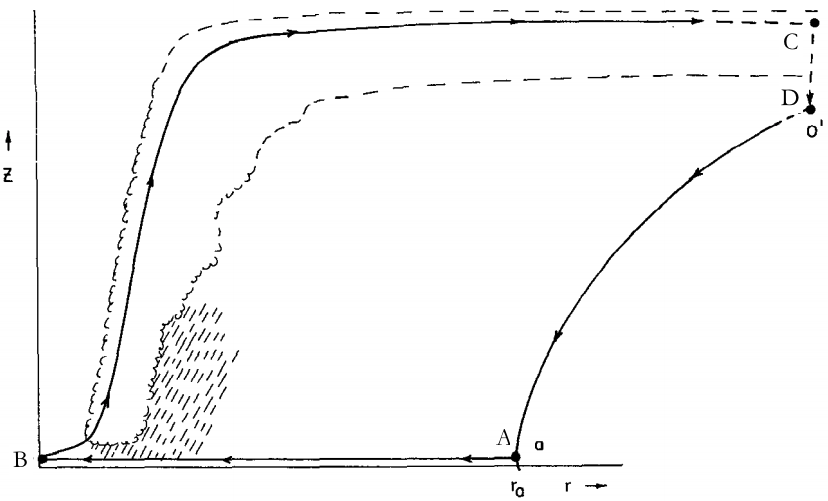
\includegraphics[width=0.49\linewidth]{images/hurricane-carnot.png}\\
    \textit{Figure 1 from~\cite{emanuel1991theory}. }
\end{figure}
\end{frame}

\begin{frame}{Cambridge Flooding Prediction~\cite{kulp2019new, kulp2018coastaldem}}
\vspace{-30pt}
\begin{figure}[htb!]
    \centering
    \hspace{-20pt}
    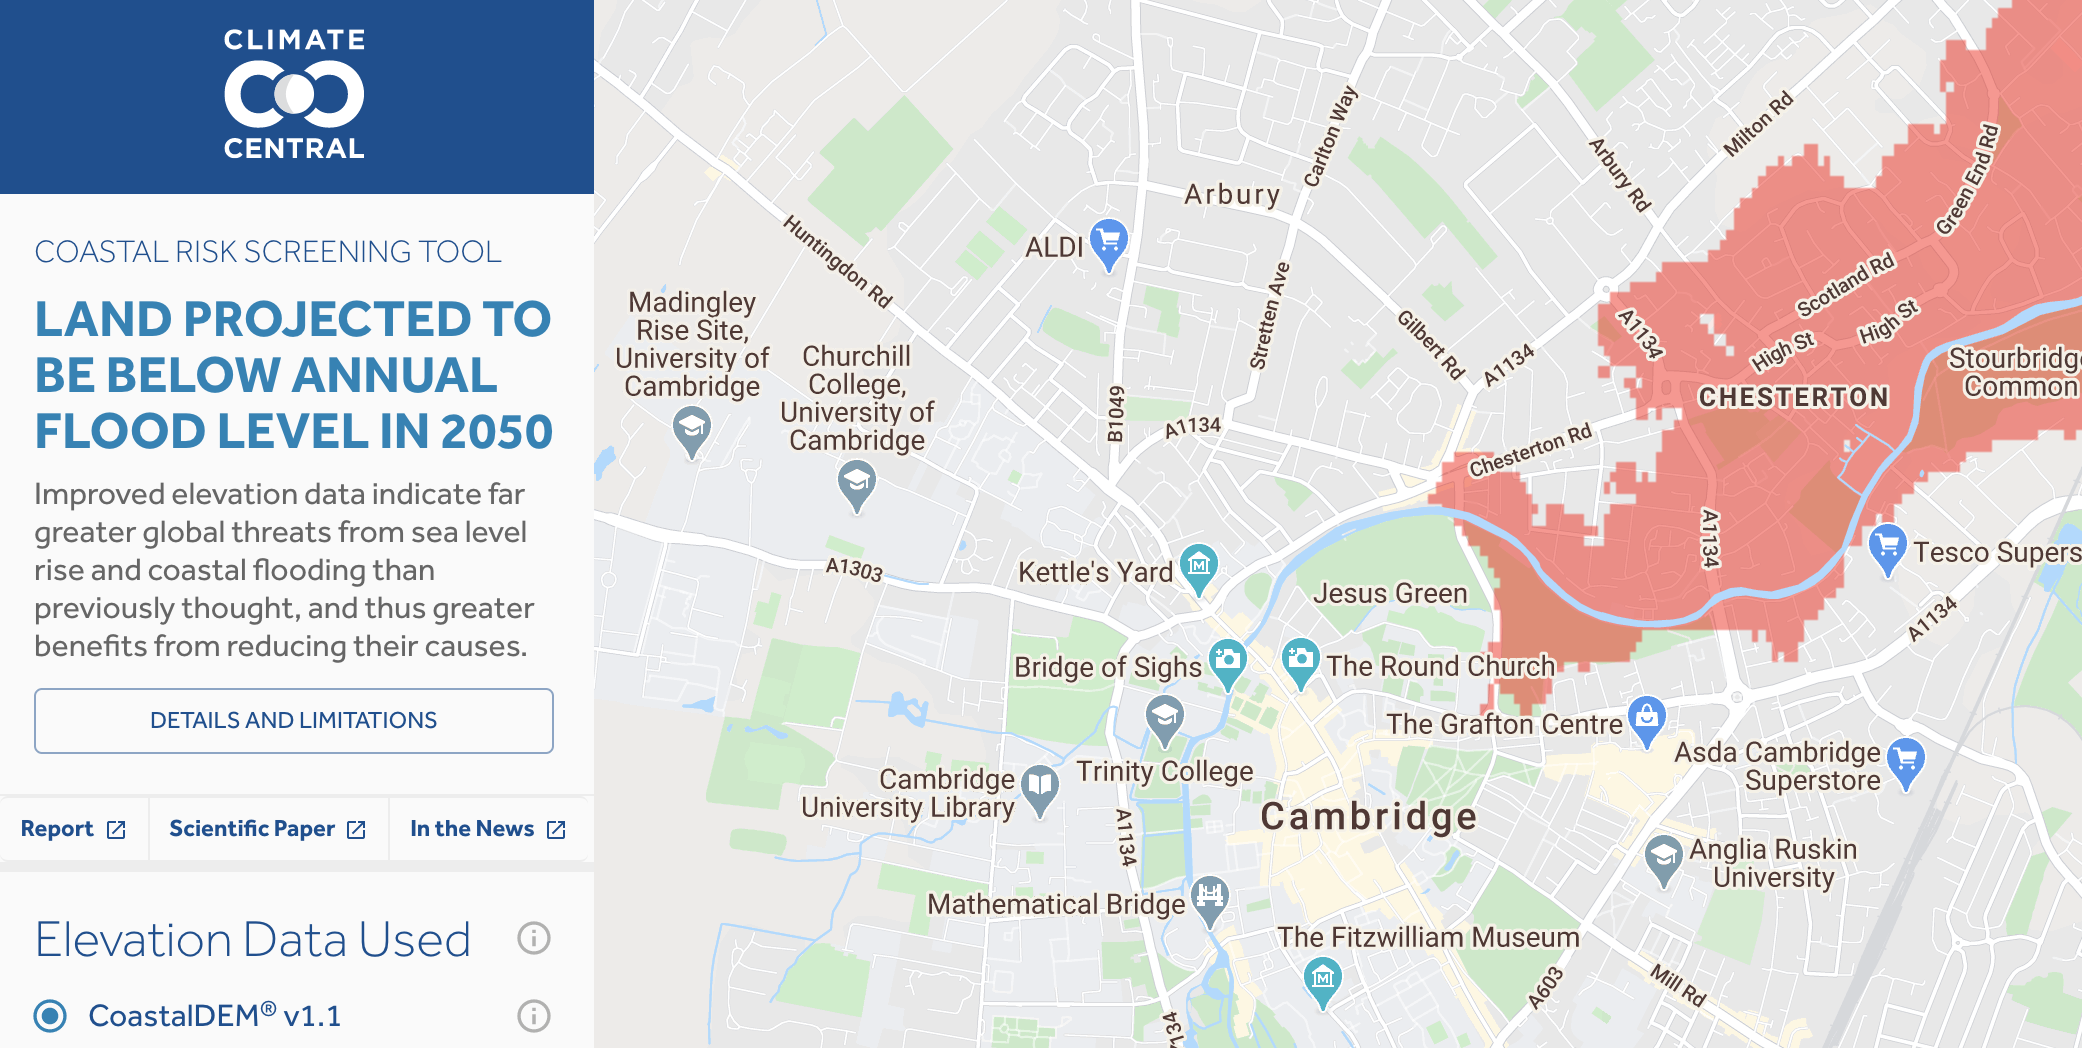
\includegraphics[width=0.9\paperwidth]{images/example-images/cambridge-surge.png}
    \vspace{-7pt}
    \caption{\url{https://coastal.climatecentral.org/map/}}
    \label{fig:}
\end{figure}
\end{frame}

\begin{frame}{New Orleans Flooding Prediction~\cite{kulp2019new, kulp2018coastaldem}}
\vspace{-20pt}
\begin{figure}[htb!]
    \centering
   \hspace{-20pt}
    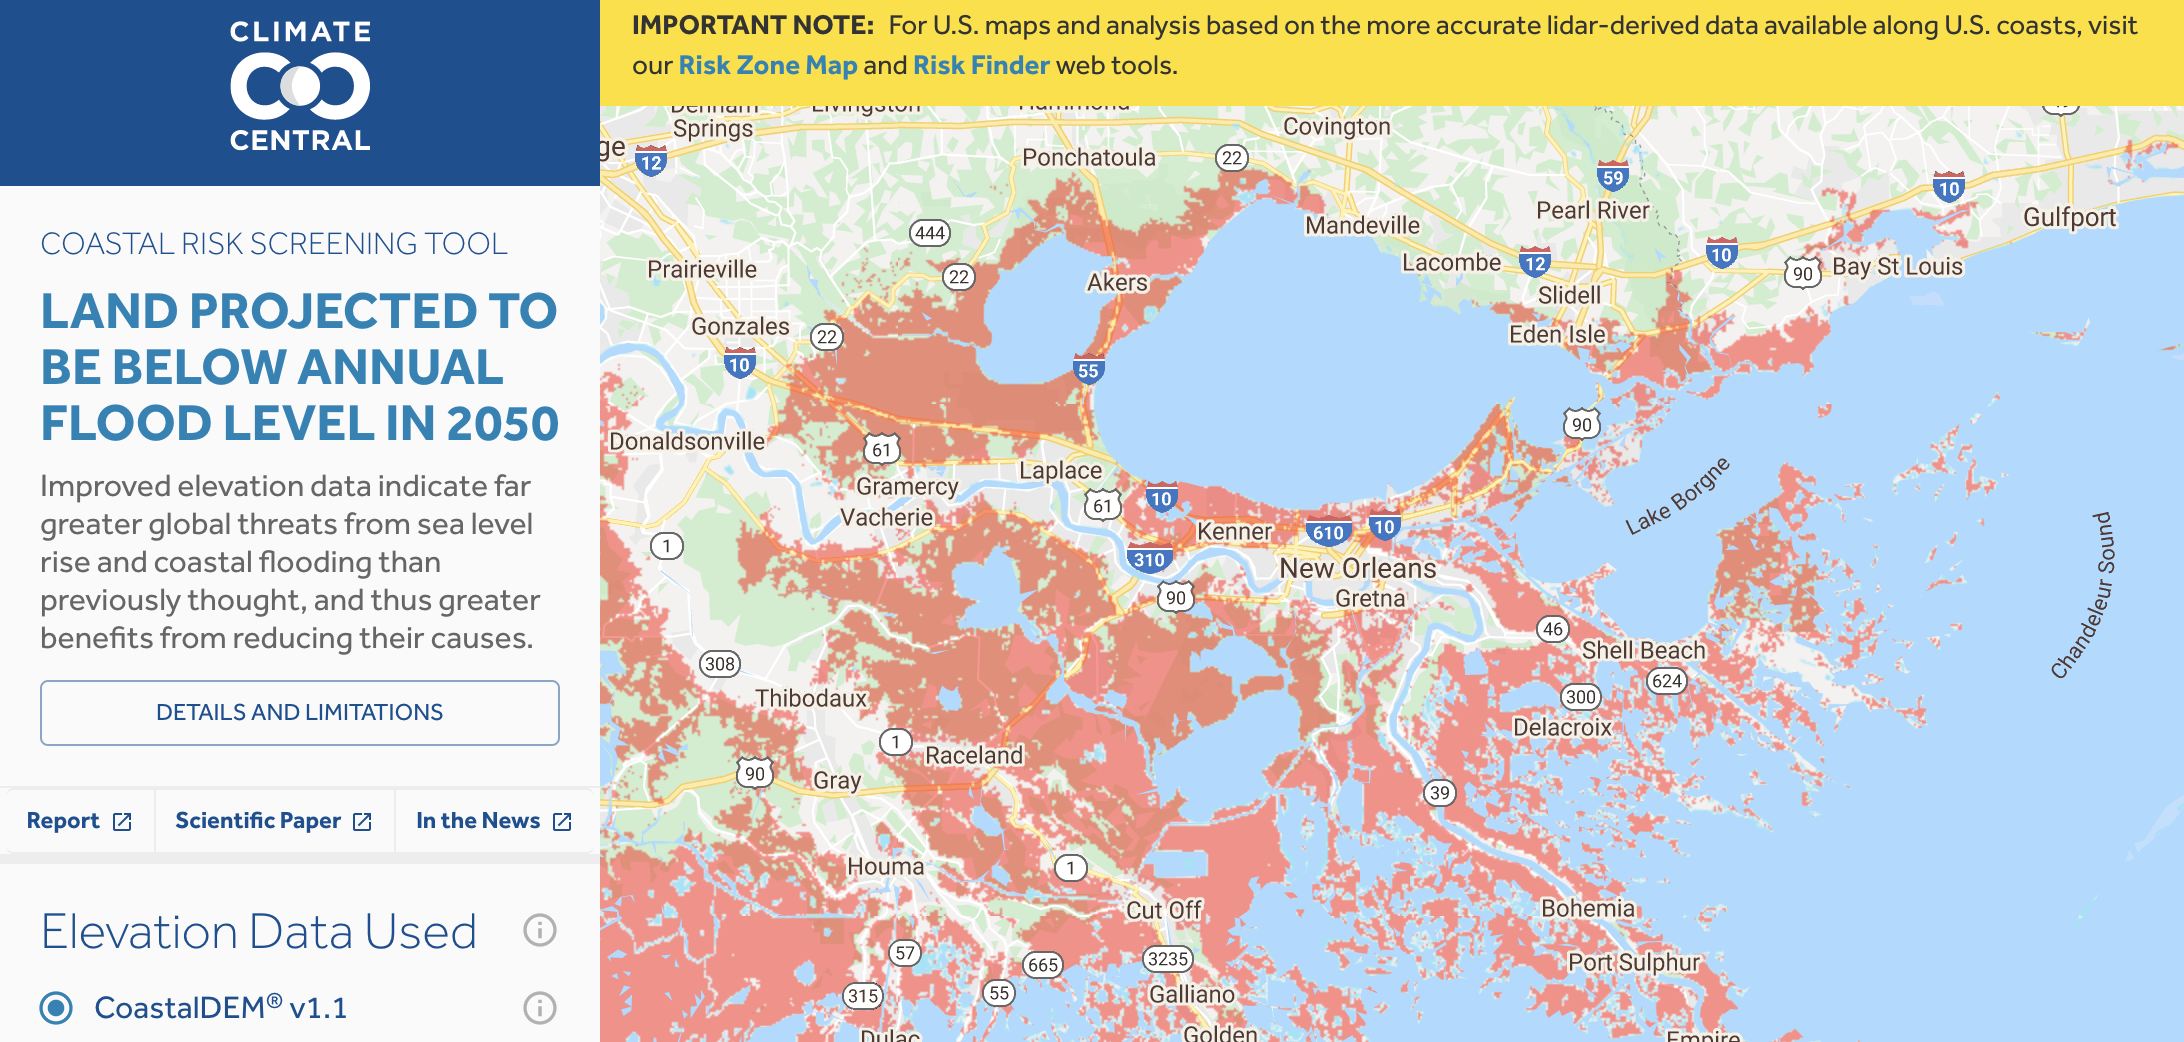
\includegraphics[width=0.9\paperwidth]{images/example-images/new-orleans-surge.png}
    \vspace{-7pt}
    \caption{\url{https://coastal.climatecentral.org/map/}}
    \label{fig:}
\end{figure}
\end{frame}

\begin{frame}{Structure}

This talk covers:
\vspace{5pt}

\begin{enumerate}
    \item A brief introduction to ORCA12 (the model used).
    \item The method of extraction of data from the model.
    \item Computing and justifying local coastal metrics.
     \item Initial local regression results.
\end{enumerate}
\begin{figure}[htb!]
    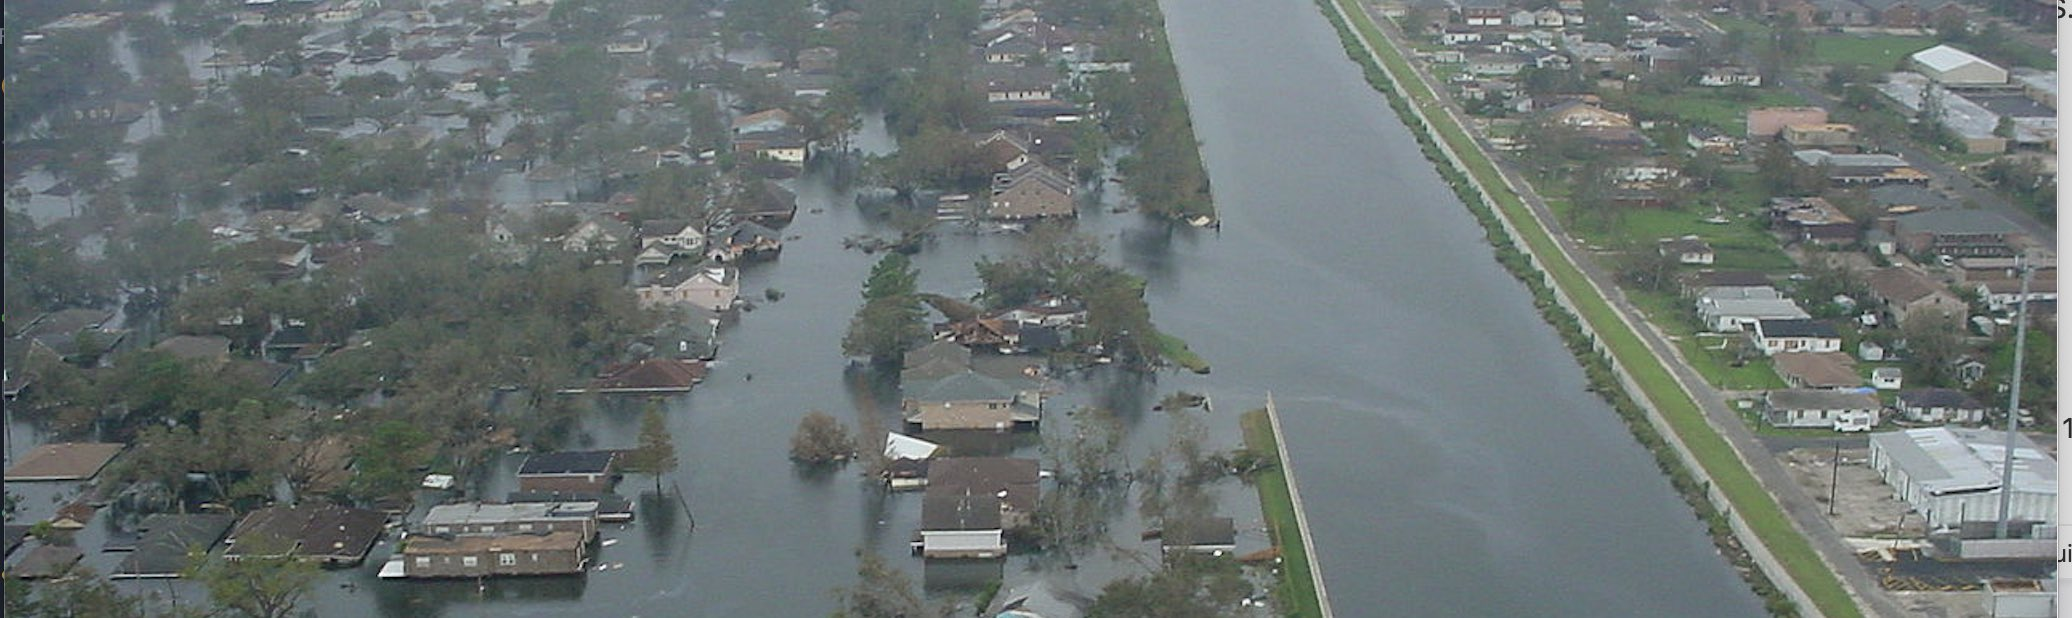
\includegraphics[width=0.9\linewidth]{images/example-images/new-orleans.jpg}
\end{figure}

This work was inspired by Yin et al.~2020~\cite{ZannaPreprint}.\\
Please contact me if you have any suggestions!
\href{mailto:sdat2@cam.ac.uk}{sdat2@cam.ac.uk}
or \href{mailto:sithom@bas.ac.uk}{sithom@bas.ac.uk}.
\begin{center}
\end{center}
\end{frame}
 

%\begin{frame}{The NEMO ORCA12 Ocean Model~\cite{madec2015nemo}}
\vspace{-20pt}
\begin{figure}[htb!]
    \centering
    \hspace{-30pt}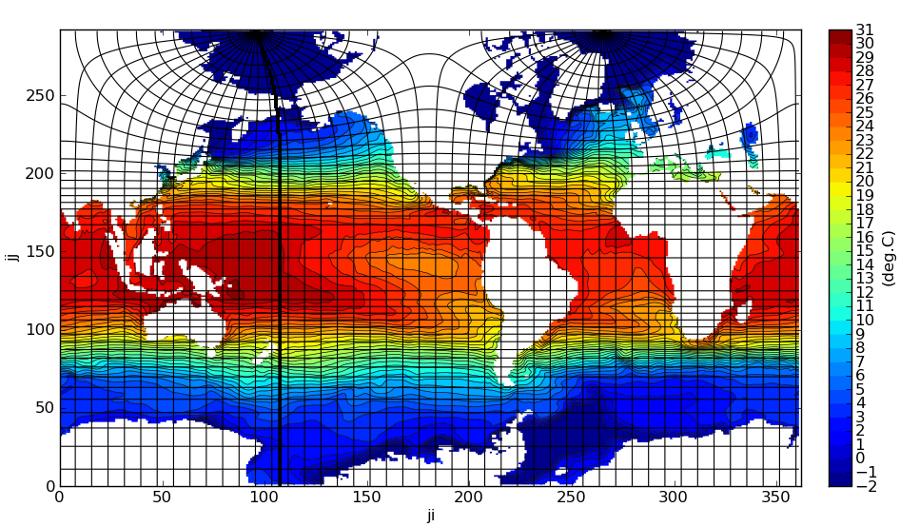
\includegraphics[width=0.74\linewidth]{images/example-images/fig-irregular.png}
     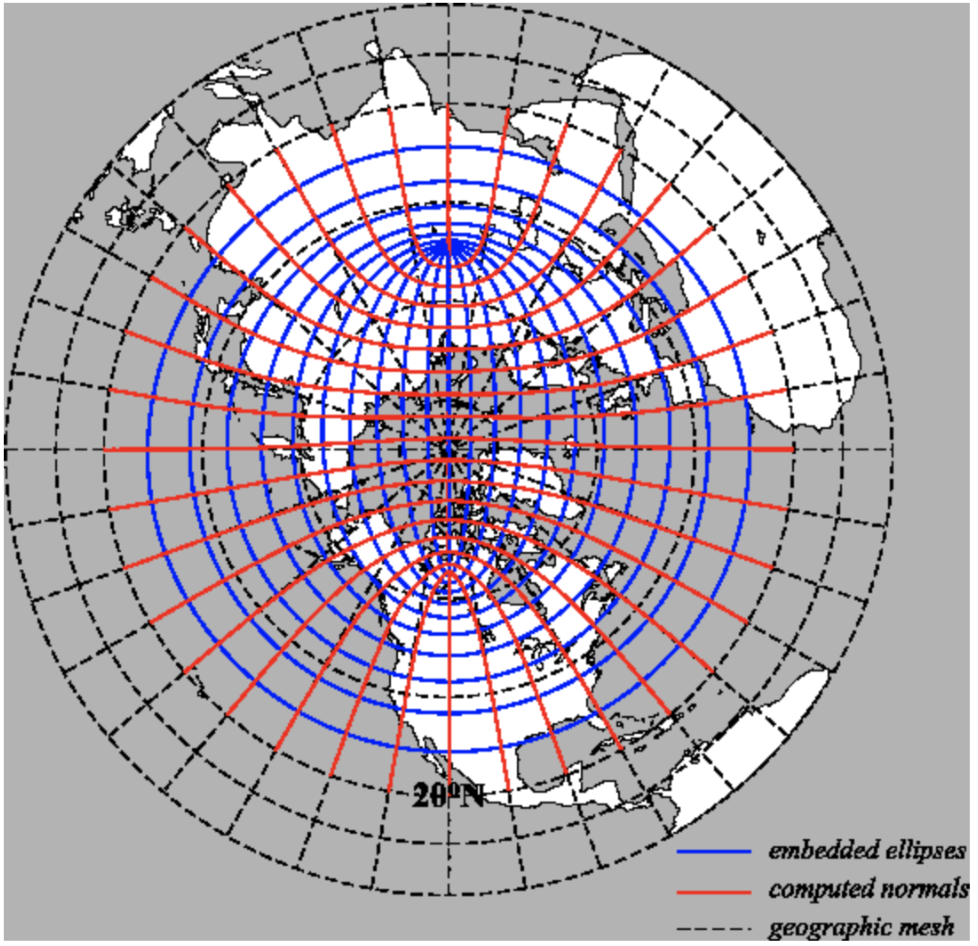
\includegraphics[width=0.30\linewidth]{images/example-images/nemo-poles.png}
    \vspace{-7pt}
    \caption{NEMO ORCA12 uses a tripolar ocean grid so that no coordinate singularities are in the ocean.
     The resolution is $\frac{1}{12}^{\circ}$.
      Initial condition EN4~\cite{good2013en4, HadObs} (start of the run = 1976).
Forcing CORE2~\cite{griffies2012datasets,large2009global}.}
    \label{fig:}
\end{figure}
\end{frame}


\begin{frame}{The HADGEM3 CMIP6 Model~\cite{williams2018met, FurtherInfo}}
\vspace{-25pt}
\begin{itemize}
\item `\texttt{control-1950}' to 2050. Daily mean outputs~\cite{williams2018met, FurtherInfo}.\footnote{\url{https://view.es-doc.org/
                                                ?renderMethod=name&project=cmip6&type=
                                                cim.2.designing.NumericalExperiment&client
                                                =esdoc-url-rewrite&name=control-1950}}

\item This experiment is not standard to CMIP6~\cite{eyring2016overview}.
\item There is a problem with representing TCs~\cite{tomassini2017interaction}:
\end{itemize}
\begin{figure}
\vspace{-18pt}
        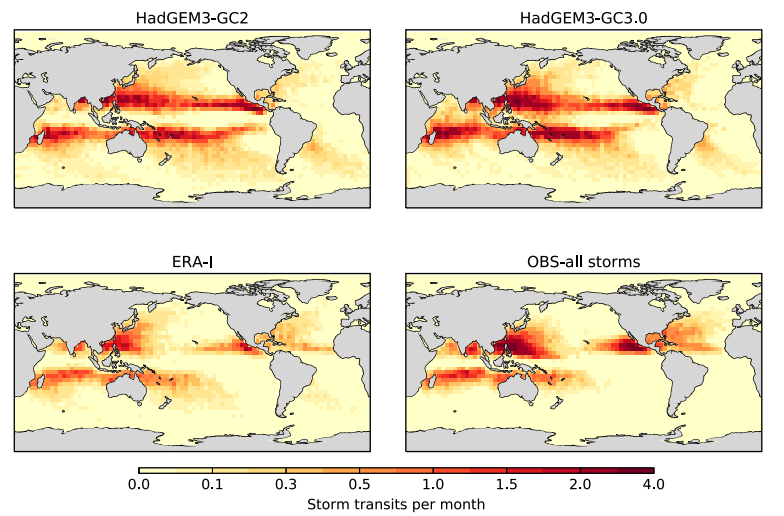
\includegraphics[width=0.7\linewidth]{images/HAD-TC.png}
\vspace{-10pt}
            \caption{The models all have
            significantly less TCs in the North Atlantic
             than observations.
             \textit{Figure 19 from~\cite{williams2018met}.} }
\end{figure}
\vspace{-15pt}
\end{frame}

\begin{frame}{Systematic Error: Wind Stress Parameterisation}
\vspace{-40pt}
\centering
\begin{equation}
 |\tau| = c_d(|U|) \cdot U^2
 \end{equation}
    \hspace{-30pt}\begin{minipage}{0.45\textwidth}
    \begin{figure}
            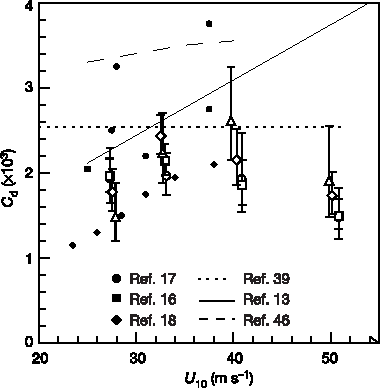
\includegraphics[width=1\linewidth]{images/example-images/cd.pdf}
                \caption{Fig. 3c from Powell 2003~\cite{powell2003reduced},
                 where they suggested that at high wind speeds $c_d$ decreases.}
    \end{figure}
    \end{minipage}\hspace{5pt}
      \begin{minipage}{0.57\textwidth}
\begin{figure}[htb!]
    \centering
    \includegraphics[width=1\linewidth]{../surge/plots/cd_finder.pdf}
    \caption{ Extracting $C_d$ from data.
    $ r_p = 0.9774 \pm 0.001,\;\; p<10^{-300}$\\
    $ m = 0.0383 \pm 0.0001 $ kg$^{0.5}$ m$^{-1.5}$\\
    $\implies  c_d = 0.001467 \pm 0.000008$ kg m$^{-3}$
    % error estimated from differences in output between test/training year,
    % measured regression error in either year much smaller than this.
    % The error is propogated using the \texttt{python3.uncertanties} package}
    }
    \label{fig:}
\end{figure}
    \end{minipage}
\end{frame}

%\begin{frame}{Helpful Place Labels}
\vspace{-20pt}
\begin{figure}[htb!]
    \centering
    \includegraphics[width=0.85\linewidth]{../surge/plots/point_choosing/standard_loc_test.pdf}
    \vspace{-7pt}
    \caption{Places that I will label the x-axis with.
     The coastline is a self-similar fractal~\cite{mandelbrot1967long, richardson1961problem},
      hence coast length is dependent on resolution.
    [Fractal dimension changes along the coast.~\cite{jiang1998fractal}]}
    \label{fig:}
\end{figure}
\end{frame}


\begin{frame}[fragile]{Automatic Point Selection}
\vspace{-20pt}

\begin{algorithm}[H]
\dontprintsemicolon
% \DontPrintSemicolon % Some LaTeX compilers require you to use \dontprintsemicolon instead
\caption{Coastal Selection}
\label{algo:Selection}
\KwIn{Grid: boolean grid (True for NaN values (land))}
\For{indices in Grid}{
  \If {Grid[indices] == False}{
     \If{ any of Grid[index\_x $\pm$ 1, index\_y $\pm$ 1] are True}
        {\textbf{append} indices to List\;}
     }
}
\KwOut{List: list of indices}
\end{algorithm}

\end{frame}

\begin{frame}[fragile]{Automatic Point Sorting}
\vspace{-20pt}
\begin{algorithm}[H]
\dontprintsemicolon
% \DontPrintSemicolon % Some LaTeX compilers require you to use \dontprintsemicolon instead
\caption{Coastal Sort}
\label{algo:Sort}
\KwIn{Input\_List: Slimmed output of Algorithm~\ref{algo:Selection}}
\KwIn{First\_Index\_Pair: Point at one end of the coast }
\KwIn{Final\_Index\_Pair: Point at other end of the coast }

\texttt{tmp} $\gets$ First\_Index\_Pair\;

\Repeat{\texttt{tmp} = Final\_Index\_Pair}{
 \textbf{append} \texttt{tmp} to Output\_List\;
 \textbf{remove} \texttt{tmp} from Input\_List\;
 \texttt{tmp} $\gets$ Input\_List[\textbf{min}$_{k}$(\textbf{distance}(\texttt{tmp}, Input\_List[k]))]\;
}
\textbf{append} Final\_Index\_Pair to Output\_List\;

\KwOut{Output\_List: sorted list of indices}
\end{algorithm}

\end{frame}


\begin{frame}{Automatically Point Selection from ORCA12}
\vspace{-20pt}
\begin{figure}[htb!]
    \centering
    \hspace{-10pt}
    \includegraphics[width=0.60\linewidth]{../surge/plots/quiver_plot.pdf}
    \hspace{5pt}
    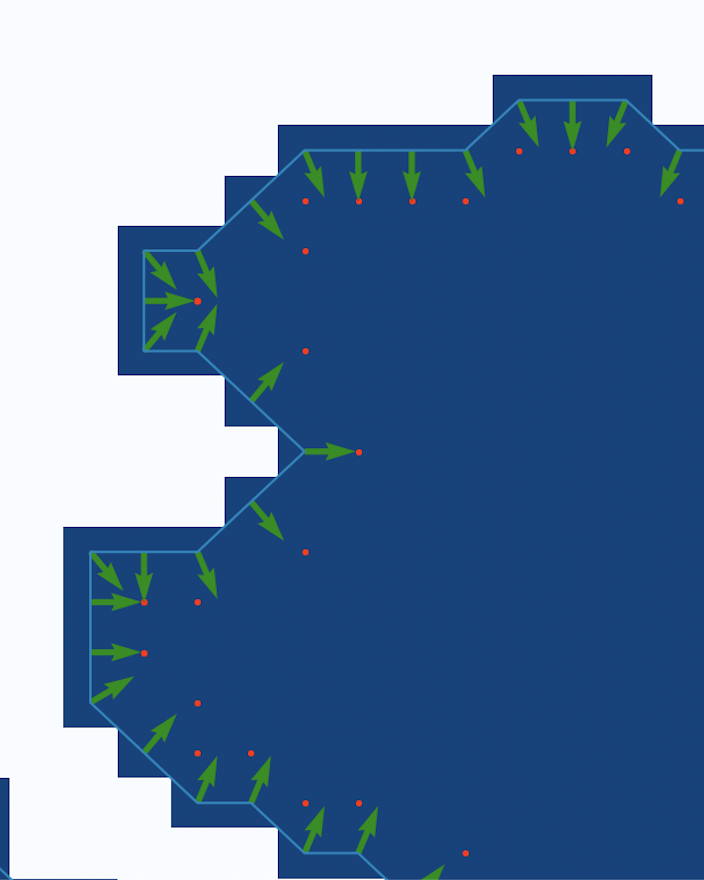
\includegraphics[width=0.38\linewidth]{images/example-images/new-orleans-example.png}
    \vspace{-7pt}
    \caption{The full selection of coastal points taken from ORCA12. Green arrows show
             orientation of that cell's stretch of coast line.}
    % \label{fig:}
\end{figure}
\end{frame}

\section{Local Coastal Metrics}
    \begin{frame}[plain]
        \vfill
      \centering
      \begin{beamercolorbox}[sep=8pt,center,shadow=true,rounded=true]{title}
        \usebeamerfont{title}\insertsectionhead\par%
        \color{oxfordblue}\noindent\rule{10cm}{1pt} \\
        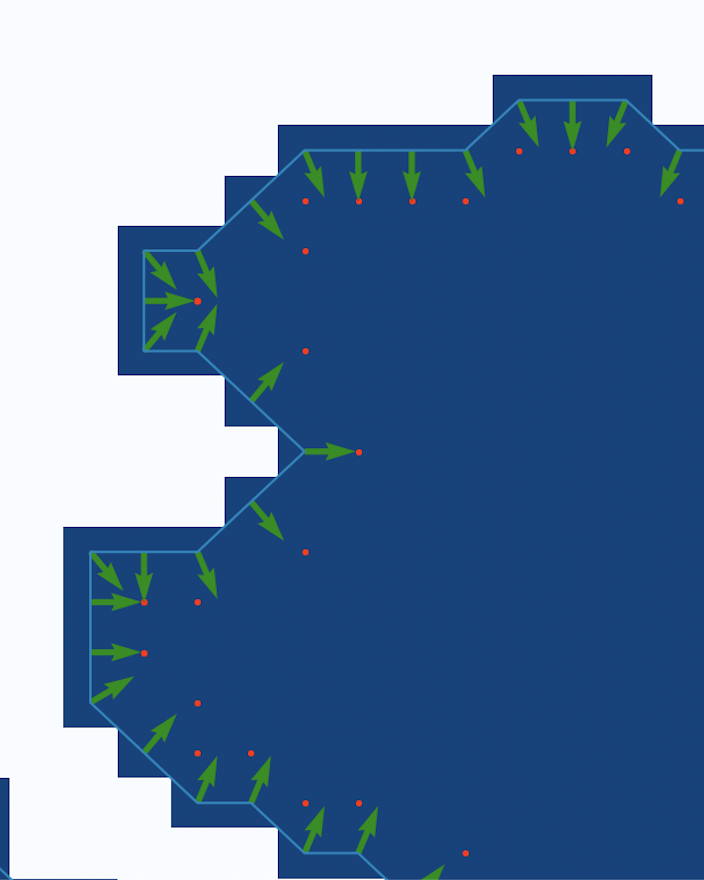
\includegraphics[width=0.4\linewidth]{images/example-images/new-orleans-example.png}
        \includegraphics[width=0.52\linewidth]{../surge/plots/angles_hist.pdf}
      \end{beamercolorbox}
      \vfill
  \end{frame}


\begin{frame}{The change in angles along the coastline}
\vspace{-20pt}
\begin{figure}[htb!]
    \centering
    \begin{equation}
B_i^{\prime}=\operatorname{arctan} 2\left(\sum_{j=i-4\sigma}^{j=i+4\sigma}
     \mathcal{N}(i, \sigma^{2})\cdot \sin{( B_{j})},\; \sum_{j=i-4\sigma}^{j=i+4\sigma}
      \mathcal{N}(i, \sigma^{2})\cdot  \cos{( B_{j})}\right)
\end{equation}
    \includegraphics[width=1.0\linewidth]{../surge/plots/angle_heatmap.pdf}
    % \caption{To deal with this we could smooth, and try a variety of $\sigma$.}
    % \label{fig:}
\end{figure}
\end{frame}


\begin{frame}{Angular derivative signal noisy for small $\sigma$}
\vspace{-20pt}
\begin{figure}[htb!]
    \centering
        \begin{equation}
        \frac{\partial B_i^{\prime}}{\partial \mathrm{pt}} \equiv \frac{B_{i+1}^{\prime}-B_{i-1}^{\prime}}{2}
\end{equation}
    \includegraphics[width=1.0\linewidth]{../surge/plots/derivative_heatmap_1_11.pdf}
    % \caption{To deal with this we could smooth, and try a variety of $\sigma$.}
    % \label{fig:}
\end{figure}
\end{frame}

%    plot_derivative_angle_heatmap(1, 11)
%    plot_derivative_angle_heatmap(10, 30)
%    plot_derivative_angle_heatmap(30, 100)

\begin{frame}{Better for  moderate $\sigma$}
\vspace{-20pt}
\begin{figure}[htb!]
    \centering
            \begin{equation}
        \frac{\partial B_i^{\prime}}{\partial \mathrm{pt}}
        \equiv \frac{B_{i+1}^{\prime}-B_{i-1}^{\prime}}{2} \notag
\end{equation}
    \includegraphics[width=1.0\linewidth]{../surge/plots/derivative_heatmap_10_30.pdf}
    % \caption{To deal with this we could smooth, and try a variety of $\sigma$.}
    % \label{fig:}
\end{figure}
\end{frame}

\begin{frame}{Unresponsive for high $\sigma$}
\vspace{-20pt}
\begin{figure}[htb!]
    \centering
\begin{equation}
        \frac{\partial B_i^{\prime}}{\partial \mathrm{pt}}
        \equiv \frac{B_{i+1}^{\prime}-B_{i-1}^{\prime}}{2} \notag
\end{equation}
    \includegraphics[width=1.0\linewidth]{../surge/plots/derivative_heatmap_30_100.pdf}
    % \caption{To deal with this we could smooth, and try a variety of $\sigma$.}
    % \label{fig:}
\end{figure}
\end{frame}


\begin{frame}{Extracting Bathymetry}
\vspace{-30pt}
\hspace{-30pt}
\begin{figure}[htb!]
    \centering
    \hspace{-30pt}\includegraphics[width=1.1\linewidth]{../surge/plots/bath_list.pdf}
    % \label{fig:}
\end{figure}
\end{frame}


\begin{frame}{Extracting Bathymetry}
\vspace{-30pt}
\hspace{-30pt}
\begin{figure}[htb!]
    \centering
    \hspace{-35pt}\includegraphics[width=1.1\linewidth]{../surge/plots/distance_isobath.pdf}
    % \label{fig:}
\end{figure}
\end{frame}

\begin{frame}{Isobath Distances are Heavily Correlated}
\vspace{-30pt}
\hspace{-30pt}
\begin{figure}[htb!]
    \centering
    \hspace{-35pt}\includegraphics[width=0.65\linewidth]{../surge/plots/isobath_correlate.pdf}
\end{figure}
\end{frame}

\begin{frame}{An Example around New Orleans}
\vspace{-30pt}
\begin{figure}[htb!]
    \centering
    \includegraphics[width=0.75\linewidth]{../surge/plots/new_orleans_map.pdf}
\end{figure}
\end{frame}

\begin{frame}{A Katrina-Like Hurricane}
\vspace{-30pt}
\begin{figure}[htb!]
    \centering
    \includegraphics[width=0.75\linewidth]{../surge/plots/katrina_graph.pdf}
\end{figure}
\end{frame}

%\section{Sea Surface Velocity along Y-axis, (Vos, $v$) }
    \begin{frame}[plain]
        \vfill
      \centering
      \begin{beamercolorbox}[sep=8pt,center,shadow=true,rounded=true]{title}
        \usebeamerfont{title}\insertsectionhead\par%
        \color{oxfordblue}\noindent\rule{10cm}{1pt} \\
        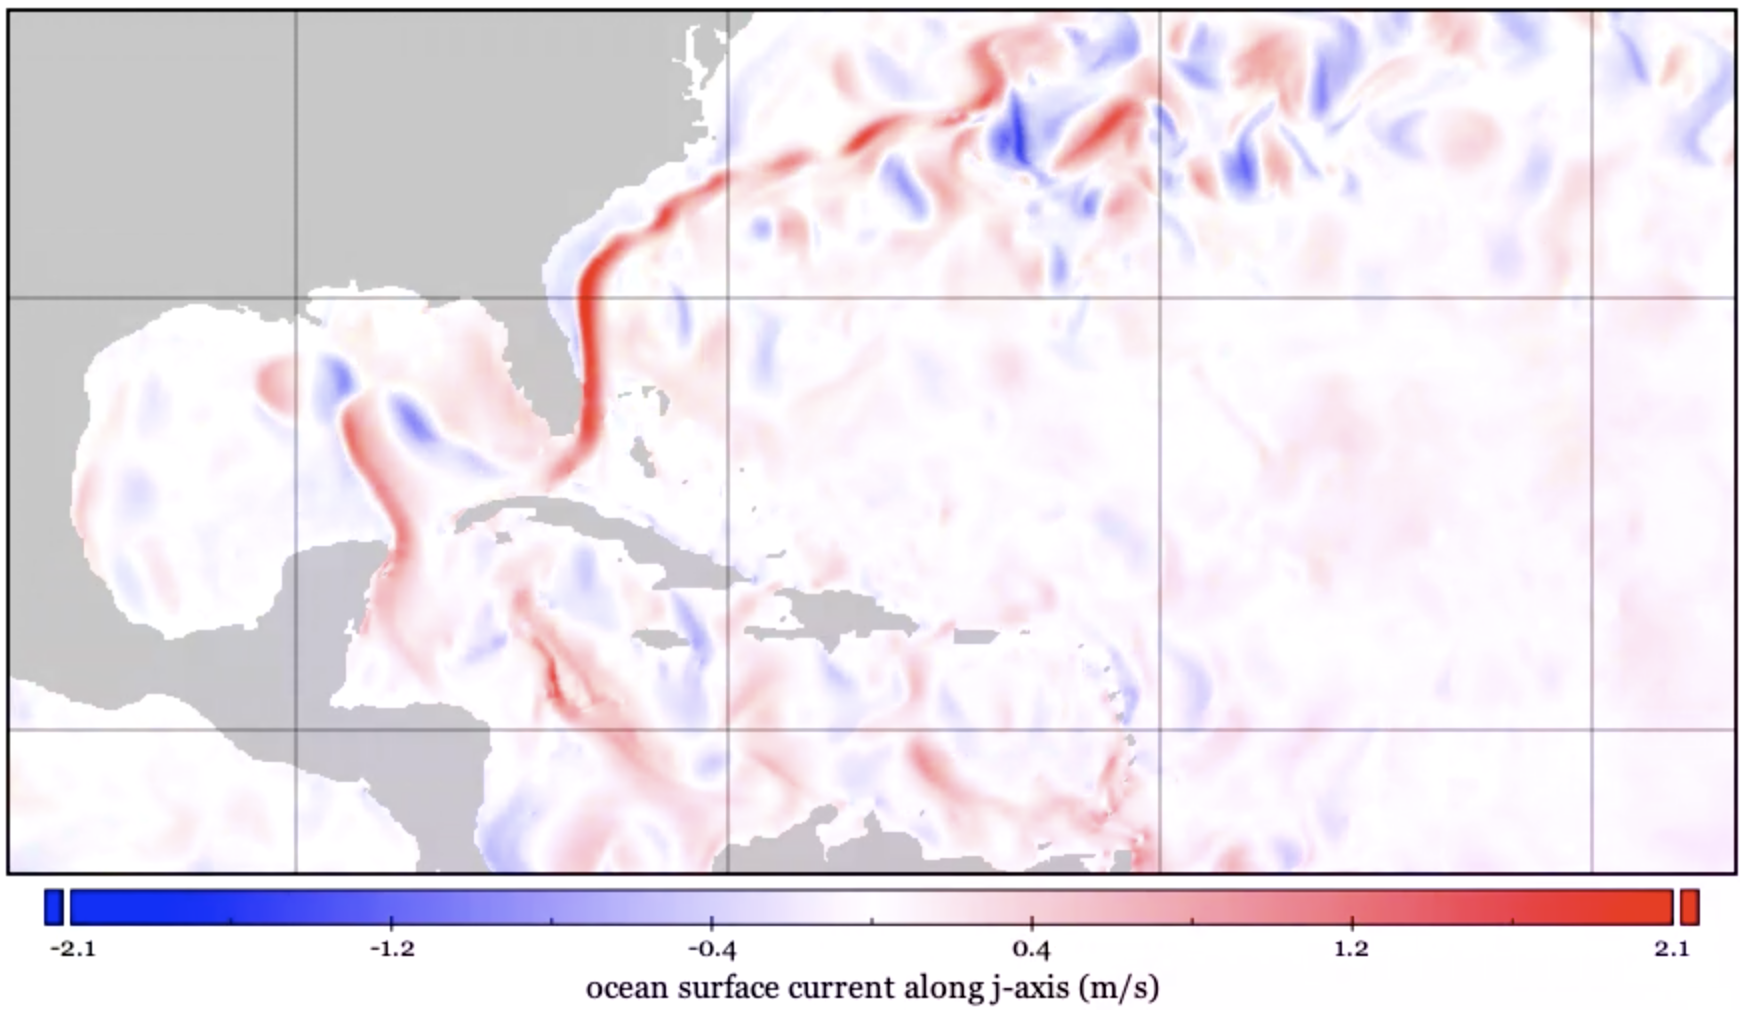
\includegraphics[width=0.93\linewidth]{images/example-images/vos.png}
      \end{beamercolorbox}
      \vfill
  \end{frame}

\section{Sea Surface Height above Reference Geoid (Zos, $\eta$, SSH) }
    \begin{frame}[plain]
        \vfill
      \centering
      \begin{beamercolorbox}[sep=8pt,center,shadow=true,rounded=true]{title}
        \usebeamerfont{title}\insertsectionhead\par%
        \color{oxfordblue}\noindent\rule{10cm}{1pt} \\
        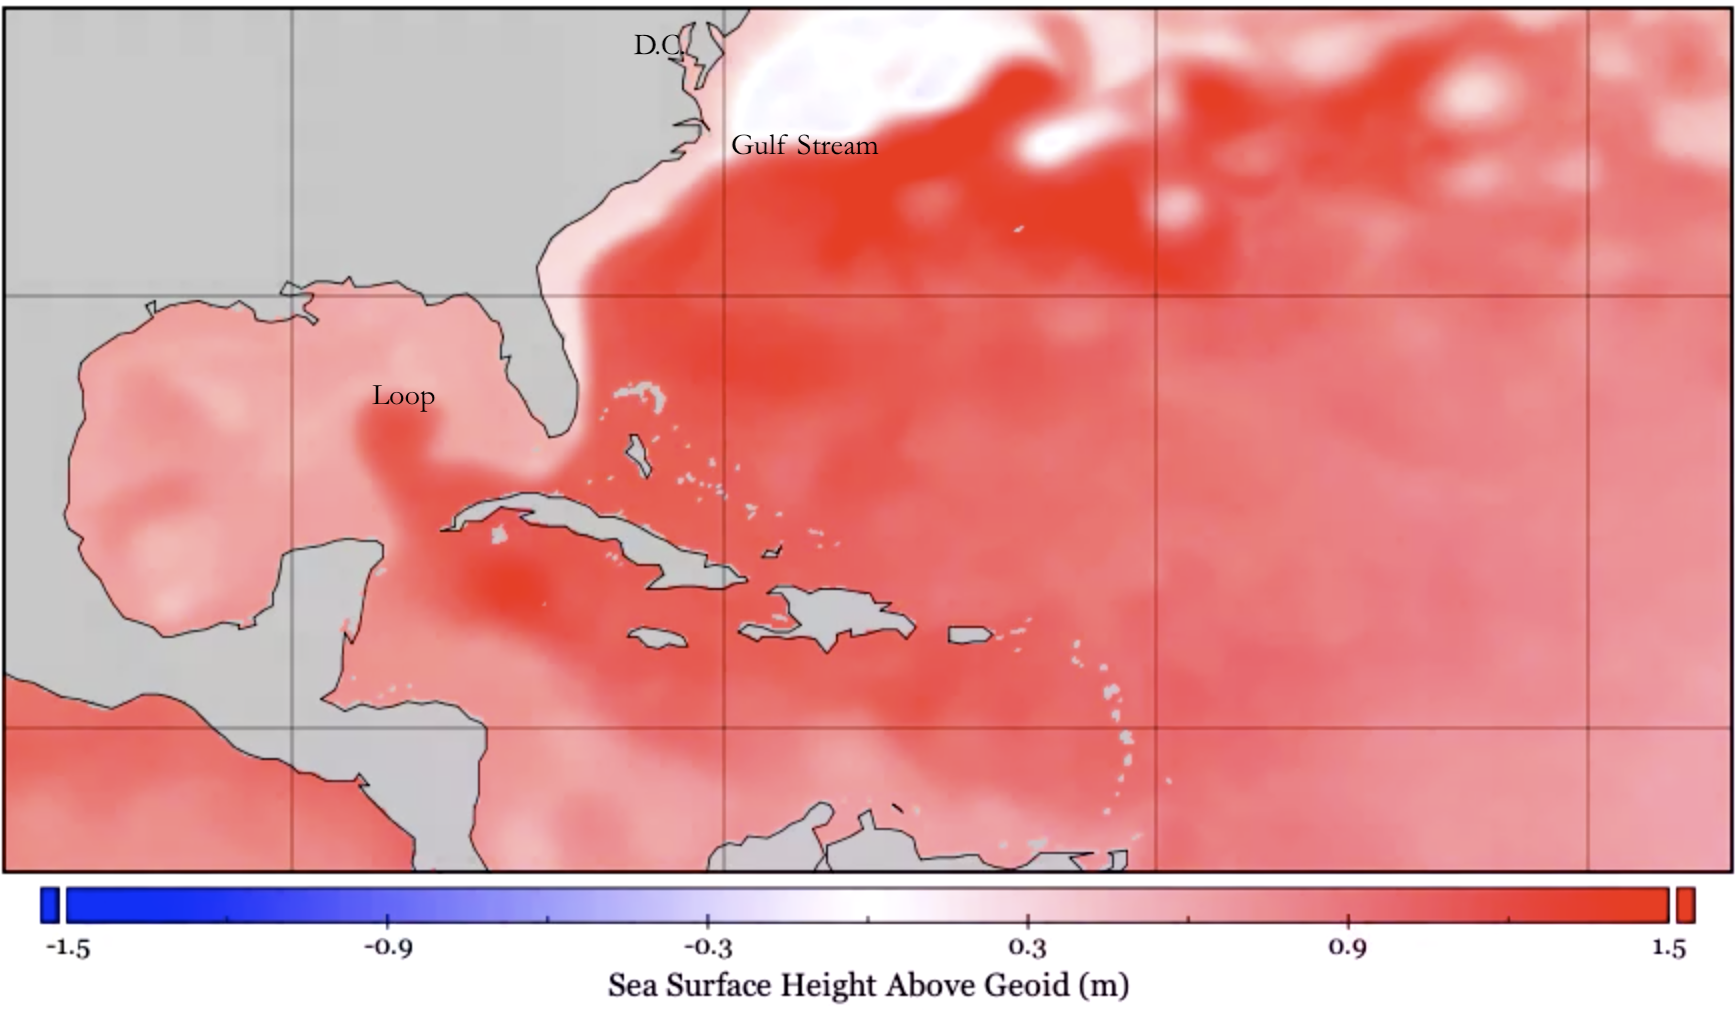
\includegraphics[width=0.93\linewidth]{images/example-images/zos-image.png}
      \end{beamercolorbox}
      \vfill
  \end{frame}

  \begin{frame}{$\eta$ Covariance and Correlation matrices are similar. }
\vspace{-20pt}
\begin{figure}[htb!]
    \centering
    \hspace{-10pt}
    \includegraphics[width=0.68\linewidth]{../surge/plots/corr_cov.pdf}
            \includegraphics[width=0.16\linewidth]{../surge/plots/corr_cov_cbar.pdf}
    \vspace{-7pt}
    \caption{A/B: Covariance matrices for 2004/5.\\
             $\quad\quad\quad\;\;$C/D: Correlation matrices for 2004/5.}
    \label{fig:}
\end{figure}
\end{frame}

\begin{frame}{ $\eta$ (SSH/zos) similar between 2004/5 }
\vspace{-20pt}
\begin{figure}[htb!]
    \centering
    \includegraphics[width=0.6\linewidth]{../surge/plots/stats_points_plot.pdf}
       \hspace{0pt} \includegraphics[width=0.285\linewidth]{../surge/plots/stats_points_plot_1.pdf}
    \vspace{-7pt}
    \caption{A comparison between the distributions of sea surface height
     above geoid (zos) for the training set (2005) and the test set (2004).}
   % \label{fig:}
\end{figure}
\end{frame}

\begin{frame}{$\eta$ No clear discontinuity between 2004/5  }
\vspace{-20pt}
\begin{figure}[htb!]
    \centering
    \includegraphics[width=0.95\linewidth]{../surge/plots/stats_points_plot_2.pdf}
    \vspace{-7pt}
    \caption{An attempt to check whether there are discontinuities
     over the special points, to explain the offsets of the means.}
    %\label{fig:}
\end{figure}
\end{frame}

\begin{frame}{Spin up may explain displacement in $\eta$ . }
\vspace{-20pt}
\begin{figure}[htb!]
    \centering
    \includegraphics[width=0.95\linewidth]{../surge/plots/stats_points_plot_5.pdf}
    \vspace{-7pt}
    \caption{Early months in 2004 do not seem
             to follow the yearly pattern followed elsewhere.}
    %\label{fig:A}
\end{figure}
\end{frame}


\begin{frame}{Gaussian Processes Refresher}
\vspace{-20pt}
\begin{itemize}
\item Equations 2.13-2.14 in GPML~\cite{williams2006gaussian}.
\begin{align}
m(\mathbf{x})&=&\mathbb{E}[f(\mathbf{x})] % \tag{Mean}
\\
k\left(\mathbf{x}, \mathbf{x}^{\prime}\right)&=&\mathbb{E}
\left[(f(\mathbf{x})-m(\mathbf{x}))\left(f\left(\mathbf{x}^{\prime}\right)
-m\left(\mathbf{x}^{\prime}\right)\right)\right]
%\tag{Covariance}
\\
f(\mathbf{x})& \sim& \mathcal{G} \mathcal{P}\left(m(\mathbf{x}),
 k\left(\mathbf{x}, \mathbf{x}^{\prime}\right)\right)%\tag{GP}
\end{align}
\item Can assume $m(\mathbf{x})=0$ without terrible consequences.
 \item Thought should be put into the form of $k\left(\mathbf{x},
  \mathbf{x}^{\prime}\right)$~\cite{duvenaud2014automatic}.
\end{itemize}
\end{frame}

\begin{frame}{Warped Gaussian Processes}
\vspace{-20pt}
\begin{itemize}
\item GPs assume that there is a Gaussian error around each point,
      but this is often not the case in real variables.
      However, it is often possible to transform to
      a space where this is the case, Krige there,
      and then transform
      back~\cite{snelson2004warped}.\footnote{\url{http://mlg.eng.cam.ac.uk/zoubin/papers/gpwarp.pdf}}
      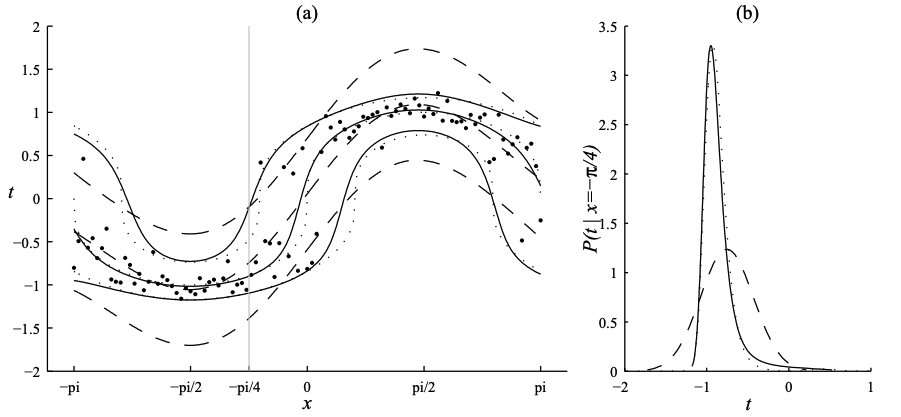
\includegraphics[width=0.7\linewidth]{images/example-images/warped-example.png}\\
      \textit{Figure 1 from~\cite{snelson2004warped}}
\item Lewis Fry Richardson (1948) showed that the estimates
      of deaths during a war had
      symmetric error bars in logarithmic space~\cite{richardson1948variation}.
      \cite{snelson2004warped}~mentions this as a common trick.
 \end{itemize}

\end{frame}


\begin{frame}{There is a strong yearly periodicity in $\eta$. }
\vspace{-20pt}
\begin{figure}[htb!]
    \centering
    \includegraphics[width=0.95\linewidth]{../surge/plots/ahh/ahhhhh4.pdf}
    \vspace{-7pt}
    \caption{There is a strong yearly periodicity in $\eta$ (and its variance?).
     Kriged with a Sobol quasirandom subsample~\cite{sobol1967distribution} of 6000 points.}
    %\label{fig:A}
\end{figure}
\end{frame}


\begin{frame}{There is  supported by taking the Fourier Transform }
\vspace{-40pt}
\begin{figure}[htb!]
    \centering
    \begin{equation}
F(f)=\int_{-\infty}^{\infty} y(x) e^{-i 2\pi f x} d x
\end{equation}
\begin{equation}
\sum_{n=0}^{N-1} a_{n} e^{-2 \pi i  k n/ N}=\sum_{n=0}^{N / 2-1} a_{2 n}
e^{-2 \pi i k (2 n)/ N} +\sum_{n=0}^{N / 2-1} a_{2n+1} e^{-2 \pi i k (2 n+1)/ N}
\end{equation}
    \includegraphics[width=0.85\linewidth]{../surge/plots/fourier_transform_grid.pdf}
    \vspace{-7pt}
    \caption{Fourier Transform~\cite{cooley1965algorithm} of $\Delta\eta$ by coastal point.}
    % \label{fig:A}
\end{figure}
\end{frame}


\begin{frame}[fragile]{Low / High Pass Filter of New Orleans }
\vspace{-10pt}
    %\centering
\begin{block}{Fast Fourier Transform (1) and Its Inverse (2)}
\vspace{-10pt}
\begin{lstlisting}[firstnumber=1, language=python, label=glabels, xleftmargin=0pt]
y(j) = (x * exp(-2*pi*sqrt(-1)*j*np.arange(n)/n)).sum()
y(j) = (x * exp(2*pi*sqrt(-1)*j*np.arange(n)/n)).mean()
\end{lstlisting}
\end{block}
\vspace{-30pt}
\begin{figure}[htb!]
\begin{equation}
\Delta\eta_{\;\mathrm{lp}}(t) = \int_{\mathbb{R}}W\left(\frac{|f|}
{|f|_{\mathrm{thresh}}}\right)\int_{\mathbb{R}}e^{2\pi i
(t-t^{\prime})f }\Delta \eta(t^{\prime})dt^{\prime}df
\end{equation}
\begin{equation}
\Delta\eta_{\;\mathrm{hp}}(t) = \int_{\mathbb{R}}\left(1-W\left(\frac{|f|}
{|f|_{\mathrm{thresh}}}\right)\right)\int_{\mathbb{R}}e^{2\pi i
(t-t^{\prime})f }\Delta \eta(t^{\prime})dt^{\prime}df
\end{equation}
    \centering
    \includegraphics[width=0.95\linewidth]{../surge/plots/norlean-low-pass.pdf}
    \vspace{-15pt}
    \caption{Fourier Transform~\cite{cooley1965algorithm} of $\Delta\eta$ for New Orleans.}
    \label{fig:A}
\end{figure}
\end{frame}

\begin{frame}[fragile]{Low / High Pass Filter of Miami }
\vspace{-10pt}
    %\centering
\begin{block}{Fast Fourier Transform (1) and Its Inverse (2)}
\vspace{-10pt}
\begin{lstlisting}[firstnumber=1, language=python, label=glabels, xleftmargin=0pt]
y(j) = (x * exp(-2*pi*sqrt(-1)*j*np.arange(n)/n)).sum()
y(j) = (x * exp(2*pi*sqrt(-1)*j*np.arange(n)/n)).mean()
\end{lstlisting}
\end{block}
\vspace{-30pt}
\begin{figure}[htb!]
\begin{equation}
\Delta\eta_{\;\mathrm{lp}}(t) = \int_{\mathbb{R}}W\left(\frac{|f|}
{|f|_{\mathrm{thresh}}}\right)\int_{\mathbb{R}}e^{2\pi i (t-t^{\prime})f }
\Delta \eta(t^{\prime})dt^{\prime}df
\end{equation}
\begin{equation}
\Delta\eta_{\;\mathrm{hp}}(t) = \int_{\mathbb{R}}\left(1-W\left(\frac{|f|}
{|f|_{\mathrm{thresh}}}\right)\right)\int_{\mathbb{R}}e^{2\pi i (t-t^{\prime})f}
   \Delta \eta(t^{\prime})dt^{\prime}df
\end{equation}
    \centering
    \includegraphics[width=0.95\linewidth]{../surge/plots/mm-low-pass.pdf}
    \vspace{-15pt}
    \caption{Fourier Transform~\cite{cooley1965algorithm} of $\Delta\eta$ for Miami.}
    \label{fig:A}
\end{figure}
\end{frame}

\begin{frame}[fragile]{Low / High Pass Filter of New York }
\vspace{-30pt}
    %\centering
\begin{block}{Fast Fourier Transform (1) and Its Inverse (2)}
\begin{lstlisting}[firstnumber=1, language=python, label=glabels, xleftmargin=0pt]
y(j) = (x * exp(-2*pi*sqrt(-1)*j*np.arange(n)/n)).sum()
y(j) = (x * exp(2*pi*sqrt(-1)*j*np.arange(n)/n)).mean()
\end{lstlisting}
\end{block}
\vspace{-20pt}
\begin{figure}[htb!]
    \centering
    \includegraphics[width=0.95\linewidth]{../surge/plots/ny-low-pass.pdf}
    \vspace{-7pt}
    \caption{Fourier Transform~\cite{cooley1965algorithm} of $\Delta\eta$ for New York.}
    \label{fig:A}
\end{figure}
\end{frame}


\begin{frame}{Low / High Pass Filter for all Points}
\vspace{-30pt}
    %\centering
\hspace{-30pt}
 \begin{minipage}{1.15\textwidth}
\begin{figure}[htb!]
    \centering
   \hspace{-40pt} \includegraphics[width=0.48\linewidth]{../surge/plots/low_pass_grid.pdf}
        \includegraphics[width=0.48\linewidth]{../surge/plots/high_pass_grid.pdf}
    \vspace{-7pt}
    \caption{Fourier Transform~\cite{cooley1965algorithm} of $\Delta\eta$}
    \label{fig:A}
\end{figure}
\end{minipage}
\end{frame}


\begin{frame}{$|f|_{thresh}=2$ yr$^{-1}$ Maximises Linear Predictability }
\centering

Linear Predictability (LP) defined in next section

    \hspace{-30pt}\begin{minipage}{0.57\textwidth}
    \begin{figure}
            \includegraphics[width=1\linewidth]{../surge/plots/reg_fft/up_to_100_full_coast.pdf}
                \caption{LP for each point.}
    \end{figure}

    \end{minipage}\hspace{5pt}
      \begin{minipage}{0.45\textwidth}
\begin{figure}[htb!]
    \centering
    \includegraphics[width=1\linewidth]{../surge/plots/reg_fft/up_to_100_coastal_average.pdf}
    \caption{Averaged over points.}
    \label{fig:}
\end{figure}
    \end{minipage}
\end{frame}

%\section{Tau-Tau Plots}
    \begin{frame}[plain]
        \vfill
      \centering
      \begin{beamercolorbox}[sep=8pt,center,shadow=true,rounded=true]{title}
        \usebeamerfont{title}\insertsectionhead\par%
        \color{oxfordblue}\noindent\rule{10cm}{1pt} \\
        \begin{itemize}
        \item As we already noted $\tau$ goes approximately quadratically with $U$.
        \item Decomposed into $\tau_u$, $\tau_v$ (along u, v axes).
        \item Regressing $\Delta\eta_{\quad hp}$ against $\tau_u$ and $\tau_v$ seems to
         reveal a linear relationship, most clear at vulnerable sights (New Orleans).
        \item How much of a difference does Robust vs. Standard Linear Regression make?
        \end{itemize}
       % 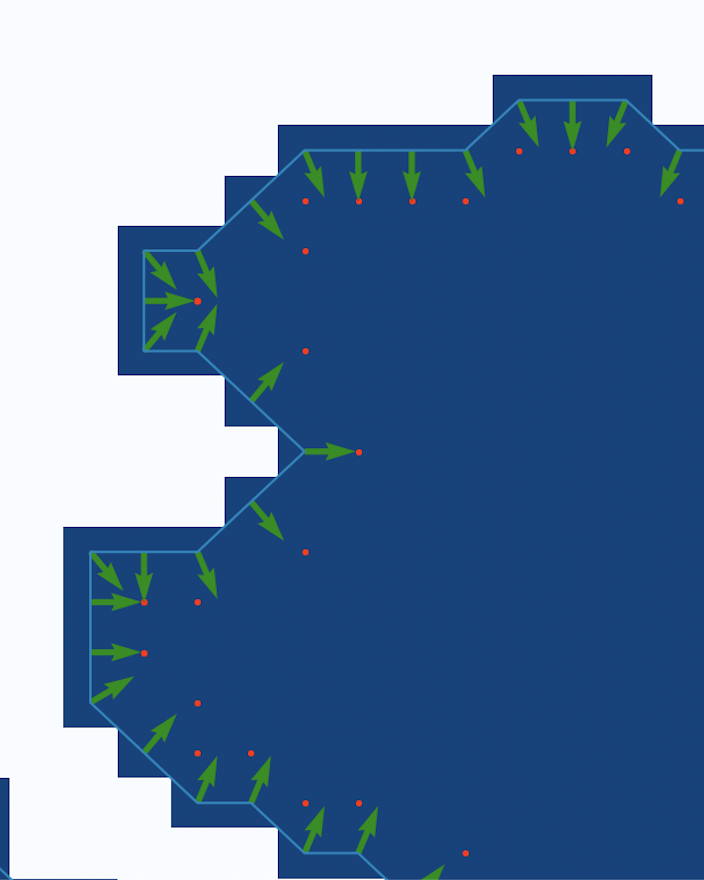
\includegraphics[width=0.4\linewidth]{images/example-images/new-orleans-example.png}
        %\includegraphics[width=0.52\linewidth]{../surge/plots/angles_hist.pdf}
      \end{beamercolorbox}
      \vfill
  \end{frame}

\begin{frame}{New Orleans $\Delta\eta$ or $\Delta\eta_{\;\;\mathrm{hp}}$ against $\tau_u$, or $\tau_v$}
\vspace{-30pt}
    %\centering
\hspace{-30pt}
 \begin{minipage}{1.15\textwidth}
\begin{figure}[htb!]
    \centering
   \hspace{-40pt} \includegraphics[width=0.42\linewidth]{../surge/plots/tau-tau/norlean-u.pdf}
        \includegraphics[width=0.42\linewidth]{../surge/plots/tau-tau/norlean-v.pdf}

   \hspace{-40pt} \includegraphics[width=0.42\linewidth]{../surge/plots/tau-tau-hp/norlean-u.pdf}
        \includegraphics[width=0.42\linewidth]{../surge/plots/tau-tau-hp/norlean-v.pdf}
    \vspace{-15pt}
    \caption{High pass filter changes New Orleans little.}
    \label{fig:A}
\end{figure}
\end{minipage}
\end{frame}

\begin{frame}{Miami $\Delta\eta$ or $\Delta\eta_{\;\;\mathrm{hp}}$ against $\tau_u$, or $\tau_v$}
\vspace{-30pt}
    %\centering
\hspace{-30pt}
 \begin{minipage}{1.1\textwidth}
\begin{figure}[htb!]
    \centering
   \hspace{-40pt} \includegraphics[width=0.42\linewidth]{../surge/plots/tau-tau/miami-u.pdf}
        \includegraphics[width=0.42\linewidth]{../surge/plots/tau-tau/miami-v.pdf}

   \hspace{-40pt} \includegraphics[width=0.42\linewidth]{../surge/plots/tau-tau-hp/miami-u.pdf}
        \includegraphics[width=0.42\linewidth]{../surge/plots/tau-tau-hp/miami-v.pdf}
    \vspace{-15pt}
    \caption{High pass filter makes Miami more New Orleans like.}
    \label{fig:A}
\end{figure}
\end{minipage}
\end{frame}


\begin{frame}{New York $\Delta\eta$ or
              $\Delta\eta_{\;\;\mathrm{hp}}$ against $\tau_u$, or $\tau_v$}
\vspace{-30pt}
    %\centering
\hspace{-30pt}
 \begin{minipage}{1.1\textwidth}
\begin{figure}[htb!]
    \centering
   \hspace{-40pt} \includegraphics[width=0.42\linewidth]{../surge/plots/tau-tau/new-york-u.pdf}
        \includegraphics[width=0.42\linewidth]{../surge/plots/tau-tau/new-york-v.pdf}

   \hspace{-40pt} \includegraphics[width=0.42\linewidth]{../surge/plots/tau-tau-hp/new-york-u.pdf}
        \includegraphics[width=0.42\linewidth]{../surge/plots/tau-tau-hp/new-york-v.pdf}
    \vspace{-15pt}
    \caption{High pass filter (lower two panels) makes small difference.}
    \label{fig:A}
\end{figure}
\end{minipage}
\end{frame}

\section{But these plots all had high excess kurtosis on all variables!  }
    \begin{frame}[plain]
        \vfill
      \centering
      \begin{beamercolorbox}[sep=8pt,center,shadow=true,rounded=true]{title}
        \usebeamerfont{title}\insertsectionhead\par%
        \color{oxfordblue}\noindent\rule{10cm}{1pt} \\
        \begin{itemize}
        \item$\mathbb{P}(\mathrm{Gaussian})<10^{-304}$ etc.
        \item The variables are also not necessarily positive (so no $\log$ trick).
        \item It would be interesting to see if there is a warping function
         that can do this (Extreme Value Textbooks are being rapidly skimmed).
        \item E.g .       \begin{equation}
       x^{\prime} = \tanh{\frac{x}{2\sigma_x}} \text{}
       \end{equation}
       Does make the distributions more normal.
        \end{itemize}
       % \includegraphics[width=0.4\linewidth]{images/example-images/new-orleans-example.png}
        %\includegraphics[width=0.52\linewidth]{../surge/plots/angles_hist.pdf}
      \end{beamercolorbox}
      \vfill
  \end{frame}


\begin{frame}{New York $\Delta\eta_{\;\;\mathrm{hp}}$ against $\tau_u$, and $\tau_v$}
\vspace{-30pt}
    %\centering
\hspace{-30pt}
 \begin{minipage}{1.1\textwidth}

\begin{figure}[htb!]
    \centering
   \hspace{-40pt} \includegraphics[width=1\linewidth]{../surge/plots/3d_plots/3d_plotnew-york.pdf}
    \vspace{-15pt}
   % \caption{High pass filter (lower two panels) makes small difference.}
    \label{fig:A}
\end{figure}
\end{minipage}
\end{frame}


\begin{frame}{Miami $\Delta\eta_{\;\;\mathrm{hp}}$ against $\tau_u$, and $\tau_v$}
\vspace{-30pt}
    %\centering
\hspace{-30pt}
 \begin{minipage}{1.1\textwidth}

\begin{figure}[htb!]
    \centering
   \hspace{-40pt} \includegraphics[width=1\linewidth]{../surge/plots/3d_plots/3d_plotmiami.pdf}
    \vspace{-15pt}
    \caption{Most variance not attributable to wind stress.}
    \label{fig:A}
\end{figure}
\end{minipage}
\end{frame}


\begin{frame}{New Orleans $\Delta\eta_{\;\;\mathrm{hp}}$ against $\tau_u$, and $\tau_v$}
\vspace{-30pt}
    %\centering
\hspace{-30pt}
 \begin{minipage}{1.1\textwidth}
\begin{figure}[htb!]
    \centering
   \hspace{-40pt} \includegraphics[width=1\linewidth]{../surge/plots/3d_plots/3d_plotnorlean.pdf}
    \vspace{-15pt}
   % \caption{High pass filter (lower two panels) makes small difference.}
    \label{fig:A}
\end{figure}
\end{minipage}
\end{frame}


\begin{frame}{Regression Summarised for Every Point.}
\vspace{-30pt}
    %\centering
\hspace{-30pt}
 \begin{minipage}{1.1\textwidth}
\begin{figure}[htb!]
    \centering
   \hspace{-40pt} \includegraphics[width=0.7\linewidth]{../surge/plots/rmlr.pdf}
    \vspace{-15pt}
   \caption{Huber regression generalises less well than MLR.}
    \label{fig:A}
\end{figure}
\end{minipage}
\end{frame}


\section{So it seems that in vulnerable places,
         a  majority of the variance can be predicted by $\tau_u$, and $\tau_v$.}
    \begin{frame}[plain]
        \vfill
      \centering
      \begin{beamercolorbox}[sep=8pt,center,shadow=true,rounded=true]{title}
        \usebeamerfont{title}\insertsectionhead\par%
        \color{oxfordblue}\noindent\rule{10cm}{1pt} \\
        \begin{itemize}
        \item Huber regression (supposedly more robust) does not significantly change the results.
        \item Approximately the same linear model is learnt, independent of year trained on.
        \item Miami, and the point near New Orleans stick out as places of poor fit.
        \end{itemize}
      \end{beamercolorbox}
      \vfill
  \end{frame}


  \begin{frame}{Orientation of the Regression Line}
\vspace{-30pt}
\hspace{-30pt}
 \begin{minipage}{1.1\textwidth}
 \begin{minipage}{0.7\textwidth}
\begin{figure}
   \hspace{-40pt} \includegraphics[width=1\linewidth]{../surge/plots/reg_angle.png}
    \vspace{-15pt}
   \caption{\texttt{np.arctan2(c0, c1)}}
    \label{fig:A}
\end{figure}
\end{minipage}
 \begin{minipage}{0.28\textwidth}
\begin{figure}[htb!]
        \vspace{-25pt}
   \hspace{-40pt} \includegraphics[width=0.95\linewidth]{../surge/plots/reg_angle_correlate.png}\\
    \hspace{-40pt} \includegraphics[width=0.95\linewidth]{../surge/plots/reg_angle_rsquare.png}
\end{figure}
\end{minipage}
\end{minipage}
\end{frame}

\section{There is a high correlation between the direction of the MLR and the
 coastline, but a specific $\sigma$ value is not picked out. }
    \begin{frame}[plain]
        \vfill
      \centering
      \begin{beamercolorbox}[sep=8pt,center,shadow=true,rounded=true]{title}
        \usebeamerfont{title}\insertsectionhead\par%
        \color{oxfordblue}\noindent\rule{10cm}{1pt} \\
        \begin{itemize}
        \item This is very gratifying, but leaves us with some problem.
        \item Increasing above $\sigma=5$ significantly increases correlation,
         suggesting that the particular orientation of the cell is not as important.
        \item The angle arrived at was also consistent between years.
        \end{itemize}
      \end{beamercolorbox}
      \vfill
  \end{frame}

\begin{frame}{The Magnitude of the  Regression Gradient.}
\vspace{-30pt}
    %\centering
\hspace{-30pt}
 \begin{minipage}{1.1\textwidth}
\begin{figure}[htb!]
    \centering
   \hspace{-40pt} \includegraphics[width=1.0\linewidth]{../surge/plots/reg_mag.pdf}
    \vspace{-15pt}
   \caption{\texttt{np.square(np.sqrt(c0) + np.sqrt(c1))}.
    This does not take account of the fact that the fits for some points are much better than others.}
    \label{fig:A}
\end{figure}
\end{minipage}
\end{frame}

\begin{frame}{Adjusted Regression Gradient.}
\vspace{-30pt}
    %\centering
\hspace{-30pt}
 \begin{minipage}{1.1\textwidth}
\begin{figure}[htb!]
    \centering
   \hspace{-40pt} \includegraphics[width=1.0\linewidth]{../surge/plots/adj_reg_mag.pdf}
    \vspace{-15pt}
   \caption{($\bar{r^2}$)\texttt{*np.square(np.sqrt(c0) + np.sqrt(c1))}. }
    \label{fig:A}
\end{figure}
\end{minipage}
\end{frame}

\begin{frame}{A reasonable $r^2$ can be produced on each.}
\vspace{-15pt}
    %\centering
\hspace{-30pt}
 \begin{minipage}{1.0\textwidth}
\begin{figure}[htb!]
    \centering
    \includegraphics[width=0.7\linewidth]{../surge/plots/ridge_lasso.pdf}
    \vspace{-15pt}
   \caption{Although not for lasso, and the regression is not consistent.
            We also need another coast to see if this generalises.}
    \label{fig:A}
\end{figure}
\end{minipage}
\end{frame}


\section{Linear Regression Algorithms (sort of) Work. }
\begin{frame}[plain]
        \vfill
      \centering
      \begin{beamercolorbox}[sep=8pt,center,shadow=true,rounded=true]{title}
        \usebeamerfont{title}\insertsectionhead\par%
        \color{oxfordblue}\noindent\rule{10cm}{1pt} \\
        \begin{itemize}
        \item Multicolinearity seems a problem in final plot.
        \item Other linear algorithms (e.g. RANSAC) could be tried
              to deal with non-normal regression.
        \item More isobath depths can be added, but this might make
              the algorithm just overfit more.
        \item Perhaps we now download the Chinese Coast from the same
              data set to see if it generalises.
        \end{itemize}
      \end{beamercolorbox}
      \vfill
\end{frame}

%\begin{frame}{Choosing the Right Comparable Area of Asia}
\vspace{-30pt}
    %\centering
\hspace{-30pt}
 \begin{minipage}{1.15\textwidth}
\begin{figure}[htb!]
    \centering
   \hspace{-40pt} \includegraphics[width=0.42\linewidth]{images/example-images/c-uos.png}
        \includegraphics[width=0.42\linewidth]{images/example-images/uos.png}

   \hspace{-40pt} \includegraphics[width=0.42\linewidth]{images/example-images/c-vos.png}
        \includegraphics[width=0.42\linewidth]{images/example-images/vos.png}
    \vspace{-10pt}
    \caption{The Kuroshio and Gulf Stream share structural features.}
    \label{fig:A}
\end{figure}
\end{minipage}
\end{frame}


\begin{frame}{Helpful Coast Markers}
\vspace{-20pt}
    %\centering
 \begin{minipage}{1.0\textwidth}
\begin{figure}[htb!]
    \centering
    \includegraphics[width=0.55\linewidth]{../surge/plots/vin-china-choice.pdf}
    \vspace{-15pt}
   \caption{Automatic coastal extraction with SH island removed. }
    %\label{fig:}
\end{figure}
\end{minipage}
\end{frame}


\begin{frame}{Algorithmic Successes}
\vspace{-20pt}
    %\centering
 \begin{itemize}
\item The nearest neighbour algorithm almost flawlessly extracted the coastline
     between two points (only Shanghai island needed to be removed by hand).
\item New documentation allowed me to speed the selection scripts up by over 3 O.M.
\item This means that selecting new areas to test theories against from ORCA12
      is now a fairly trivial undertaking.
\end{itemize}
\end{frame}

\begin{frame}{VC GEV Distribution fitted to Block Maxima}
\vspace{-20pt}
    %\centering
\begin{figure}
\includegraphics[width=0.8\linewidth]{../surge/plots/vc_skextreme_second_tactic.pdf}
\caption{\cite{skextremes} }
\end{figure}
\end{frame}


\begin{frame}{VC $\eta$ (SSH/zos) similar between 2004/5 }
\vspace{-20pt}
\begin{figure}[htb!]
    \centering
    \includegraphics[width=0.6\linewidth]{../surge/plots/vc_stats/zos_moments.pdf}
       \hspace{0pt} \includegraphics[width=0.285\linewidth]{../surge/plots/vc_stats/zos_moments_dist.pdf}
    \vspace{-7pt}
    \caption{A comparison between the distributions of sea surface height
     above geoid (zos) for the training set (2005) and the test set (2004).}
   % \label{fig:}
\end{figure}
\end{frame}



\begin{frame}{VC $\eta$ Covariance and Correlation matrices. }
\vspace{-20pt}
\begin{figure}[htb!]
  \centering
  \hspace{-10pt}
  \includegraphics[width=0.68\linewidth]{../surge/plots/vc_stats/zos_corr_cov.pdf}
          \includegraphics[width=0.165\linewidth]{../surge/plots/corr_cov_cbar.pdf}
  \vspace{-7pt}
  \caption{A/B: Covariance matrices for 2004/5.\\
           $\quad\quad\quad\;\;$C/D: Correlation matrices for 2004/5.}
  \label{fig:}
\end{figure}
\end{frame}


\begin{frame}{VC $\tau_u$ Covariance and Correlation matrices. }
\vspace{-20pt}
\begin{figure}[htb!]
  \centering
  \hspace{-10pt}
  \includegraphics[width=0.68\linewidth]{../surge/plots/vc_stats/tauuo_corr_cov.pdf}
          \includegraphics[width=0.165\linewidth]{../surge/plots/corr_cov_cbar.pdf}
  \vspace{-7pt}
  \caption{A/B: Covariance matrices for 2004/5.\\
           $\quad\quad\quad\;\;$C/D: Correlation matrices for 2004/5.}
  \label{fig:}
\end{figure}
\end{frame}

\begin{frame}{VC $\eta$ Individual Points. }
\vspace{-20pt}
\begin{figure}[htb!]
  \centering
  \hspace{-10pt}
  \includegraphics[width=1\linewidth]{../surge/plots/vc_stats/zos_individual.pdf}
  \vspace{-7pt}
  \caption{There is a lack of large positive anomalies. I don't understand what
   produces so many negative anomalies further North.}
  \label{fig:}
\end{figure}
\end{frame}


\begin{frame}{VC Bathymetry. }
\vspace{-20pt}
\begin{figure}[htb!]
  \centering
  \hspace{-10pt}
  \includegraphics[width=1\linewidth]{../surge/plots/vc_bath_list.pdf}
  \vspace{-7pt}
  \caption{}
  \label{fig:}
\end{figure}
\end{frame}


\begin{frame}{VC Bathymetry. }
\vspace{-20pt}
\begin{figure}[htb!]
  \centering
  \hspace{-10pt}
  \includegraphics[width=1\linewidth]{../surge/plots/vc_distance_isobath.pdf}
  \vspace{-7pt}
  %\caption{}
  \label{fig:}
\end{figure}
\end{frame}

\begin{frame}{VC Angles. }
\vspace{-20pt}
\begin{figure}[htb!]
  \centering
  \hspace{-10pt}
  \includegraphics[width=1\linewidth]{../surge/plots/vc_angle_heatmap.pdf}
  \vspace{-7pt}
  \label{fig:}
\end{figure}
\end{frame}


\begin{frame}{Better for  moderate $\sigma$}
\vspace{-20pt}
\begin{figure}[htb!]
    \centering
            \begin{equation}
        \frac{\partial B_i^{\prime}}{\partial \mathrm{pt}}
        \equiv \frac{B_{i+1}^{\prime}-B_{i-1}^{\prime}}{2} \notag
\end{equation}
    \includegraphics[width=1.0\linewidth]{../surge/plots/vc_derivative_heatmap_10_30.pdf}
    % \caption{To deal with this we could smooth, and try a variety of $\sigma$.}
    % \label{fig:}
\end{figure}
\end{frame}


\begin{frame}{VC Responsiveness}
\vspace{-20pt}
\begin{figure}[htb!]
    \centering
    \includegraphics[width=0.8\linewidth]{../surge/plots/vc_rmlr.pdf}
    % \label{fig:}
\end{figure}
\end{frame}

\begin{frame}{VC Responsiveness}
\vspace{-20pt}
\begin{figure}[htb!]
    \centering
    \includegraphics[width=0.8\linewidth]{../surge/plots/vc_ridge_lasso.pdf}
    % \label{fig:}
\end{figure}
\end{frame}


\begin{frame}{VC Low / High Pass Filter for all Points}
\vspace{-30pt}
    %\centering
\hspace{-30pt}
 \begin{minipage}{1.15\textwidth}
\begin{figure}[htb!]
    \centering
   \hspace{-40pt} \includegraphics[width=0.48\linewidth]{../surge/plots/vc_low_pass_grid.pdf}
        \includegraphics[width=0.48\linewidth]{../surge/plots/vc_high_pass_grid.pdf}
    \vspace{-7pt}
    \caption{Fourier Transform~\cite{cooley1965algorithm} of $\Delta\eta$.}
    % \label{fig:A}
\end{figure}
\end{minipage}
\end{frame}

%\section{Extreme Value Theory. }
\begin{frame}[plain]
        \vfill
      \centering
      \begin{beamercolorbox}[sep=8pt,center,shadow=true,rounded=true]{title}
        \usebeamerfont{title}\insertsectionhead\par%
        \color{oxfordblue}\noindent\rule{10cm}{1pt} \\
        \begin{itemize}
        \item Normal Choices are POT or Block Maxima, but these strategies require
              large amounts of data to converge~\cite{taleb2019much}.
        \item \texttt{skextreme}~\cite{skextremes} is an python package that implements these
              standard strategies.
        \item Taleb does present some solutions~\cite{taleb2019statistical}.
        \item As physical processes with understood causes, TCs
              and their storm surges are \texttt{grey not black swans}.
        \item Need to know bias between hourly to daily output.
        \end{itemize}
      \end{beamercolorbox}
      \vfill
\end{frame}


\begin{frame}{Initial Block Maxima EVT }
\begin{itemize}
    \item The Block Maxima method with the ORCA12
    \texttt{control-1950} seemed easier to initially implement.
    \item Whether POT or BM converges faster depends
          on the underlying distribution~\cite{bucher2018horse}.
    \item The input is the 101 yearly maxima for each of the points along the coast,
         relative to the deviation from the long term mean.
    \item I initially use two different BM modules in \texttt{skextreme}.
    \end{itemize}
    \end{frame}
    \begin{frame}{GEV Equations }
    \begin{itemize}
\item
\(
\operatorname{GEV}(\mu, \sigma, \xi):
\)
\(
\text{ location, } \mu \in \mathbb{R}
\text{; scale, } \sigma>0
\text{; shape, } \xi \in \mathbb{R}.
\)
\begin{eqnarray}
\operatorname{GEV}(x; \mu, \sigma, \xi)=&
\frac{1}{\sigma} \chi(x)^{\xi+1} e^{-\chi(x)};\\
\chi(x)=&\left\{\begin{array}{ll}
\left(1+\xi\left(\frac{x-\mu}{\sigma}\right)\right)^{-1 / \xi} & \text { if } \xi \neq 0 \\
e^{-(x-\mu) / \sigma} & \text { if } \xi=0
\end{array}\right.
\end{eqnarray}
\item The Gumbel distribution is a special case ($\xi=0$)

\begin{equation} \operatorname{GUM}(x ; \mu, \sigma)=e^{-\frac{x-\mu}{\sigma}-e^{-(x-\mu) / \sigma}}
\end{equation}
\end{itemize}
\end{frame}


\begin{frame}{Leiblein New Orleans}
\vspace{-20pt}
    %\centering
 \begin{minipage}{1.0\textwidth}
\begin{figure}[htb!]
    \centering
    \includegraphics[width=1\linewidth]{../surge/plots/Lieblein_modelNO.pdf}
    \vspace{-15pt}
   \caption{Interesting transition - does this represent hurricanes? }
    \label{fig:}
\end{figure}
\end{minipage}
\end{frame}


\begin{frame}{Leiblein Miami}
\vspace{-20pt}
    %\centering
 \begin{minipage}{1.0\textwidth}
\begin{figure}[htb!]
    \centering
    \includegraphics[width=1\linewidth]{../surge/plots/Lieblein_modelMM.pdf}
    \vspace{-15pt}
   \caption{Fits Line well. }
    \label{fig:}
\end{figure}
\end{minipage}
\end{frame}


\begin{frame}{Leiblein Along Coast}
\vspace{-20pt}
    %\centering
 \begin{minipage}{1.0\textwidth}
\begin{figure}[htb!]
    \centering
    \includegraphics[width=1\linewidth]{../surge/plots/skextreme_first_tactic.pdf}
    \vspace{-15pt}
   \caption{. }
    \label{fig:}
\end{figure}
\end{minipage}
\end{frame}


\begin{frame}{GEV New Orleans}
\vspace{-20pt}
    %\centering
 \begin{minipage}{1.0\textwidth}
\begin{figure}[htb!]
    \centering
    \includegraphics[width=1\linewidth]{../surge/plots/GEV_modelNO.pdf}
    \vspace{-15pt}
   \caption{. }
    \label{fig:}
\end{figure}
\end{minipage}
\end{frame}

\begin{frame}{GEV Miami}
\vspace{-20pt}
    %\centering
 \begin{minipage}{1.0\textwidth}
\begin{figure}[htb!]
    \centering
    \includegraphics[width=1\linewidth]{../surge/plots/GEV_modelMM.pdf}
    \vspace{-15pt}
   \caption{. }
    \label{fig:}
\end{figure}
\end{minipage}
\end{frame}

\begin{frame}{GEV Models Along Coast}
\vspace{-20pt}
    %\centering
 \begin{minipage}{1.0\textwidth}
\begin{figure}[htb!]
    \centering
    \includegraphics[width=1\linewidth]{../surge/plots/skextreme_second_tactic.pdf}
    \vspace{-15pt}
   \caption{. }
    \label{fig:}
\end{figure}
\end{minipage}
\end{frame}


\begin{frame}{There is a physical maximum given the climatology.}

\vspace{-30pt}
\begin{figure}[htb!]
    \centering
    \includegraphics[width=0.8\linewidth]{images/hurricane-Emanuel-upper-bound.png}
    \vspace{-15pt}
   \caption{\cite{emanuel1987dependence} }
    \label{fig:}
\end{figure}
\end{frame}

\begin{frame}{So could we do something more intelligent?~\cite{taleb2019statistical}}
\vspace{-20pt}
    %\centering
 \begin{minipage}{1.0\textwidth}
\begin{figure}[htb!]
    \centering
    \includegraphics[width=1\linewidth]{images/nnt-upper-bound.png}
    \vspace{-15pt}

   %\caption{. }
    % \label{fig:}
\end{figure}
\end{minipage}
\end{frame}

%\begin{frame}{Summary}
\begin{itemize}
\item The picture revealed by our current results broadly agrees well with that
      of~\cite{ZannaPreprint}, despite the current model being twenty four times
      the temporal resolution, and three times the lateral resolution.
%\item However each year of data does not fully sample the distribution
       (I mean that there can't be the expected fractional number of storms
        in a location in a year), but there may be ways around this.
\item As the coast is a self-similar fractal~\cite{mandelbrot1967long, richardson1961problem},
      it is unclear which length scale to average over to find summary statistics
      for a point on the coast. A reasonable solution would be to give the
      regression algorithm a number of these, and make it decide what is relevant.
\end{itemize}

\end{frame}

\begin{frame}{Current Priorities}
\begin{itemize}
\item Refine measure of the responsiveness  (storm efficiency in~\cite{ZannaPreprint})
      of a coastline unit to a wind stress event.
\item Try to untangle the contribution of
	    convexity, and bathymetry to the responsiveness.
\end{itemize}
\end{frame}

\begin{frame}{Thank you for listening!}
      \begin{minipage}{1.1\textwidth}
   \hspace{-20pt}\begin{minipage}{0.45\textwidth}
   \textbf{Resources Used:}
   \begin{itemize}
\item \texttt{matplotlib}~\cite{Hunter:2007} for original figures,
\item WebPlotDigitiser~\cite{WebPlotDigitiser} for data extraction,
\item Mathpix~\cite{mathpix} for maths extraction,
\item sci-kit-learn~\cite{scikit-learn}  for ML,
\item \texttt{cmocean}~\cite{thyng2016true}
for cmaps,
\item \texttt{numba.jit}~\cite{lam2015numba} for speed,
\item \texttt{uncertainties}~\cite{lebigot2010uncertainties} for error propogation,
\item \texttt{xarray}~\cite{hoyer2017xarray} for ND~data.
\end{itemize}
    \end{minipage}\hspace{10pt}
      \begin{minipage}{0.50\textwidth}
    \begin{figure}
            \includegraphics[width=1\linewidth]{images/example-images/Compared_O2.pdf}
            \normalsize{
    %$\tau=5.71\pm0.15\;\mathrm{yrs},\quad$\\
    $\implies \mathrm{t}_{\mathrm{double}}=4.0\pm0.1\;\mathrm{yrs}$}
                \caption{The number of papers ($\mathrm{N}$) with keyword ML
                 has increased exponentially over the last 25 years.\\ \textit{
                   Data Source: Web of Science.} %~\cite{WOS}
                   }
    \end{figure}
    \end{minipage}
\end{minipage}
\end{frame}

%
\begin{frame}{SSH SST}
\vspace{-20pt}
\begin{figure}
\includegraphics[width=0.8\linewidth]{../surge/plots/temp/ssh_sst_grid.pdf}
\caption{}
\end{figure}
\end{frame}


\begin{frame}{Demeaned}
\vspace{-20pt}
\begin{figure}
\includegraphics[width=0.8\linewidth]{../surge/plots/temp/dm_zos_dm_tos.pdf}
\caption{}
\end{figure}
\end{frame}


\begin{frame}{Low Pass of Both (threshold = 2 yr$^{-1}$ )}
\vspace{-20pt}
\begin{figure}
\includegraphics[width=0.8\linewidth]{../surge/plots/temp/lp_zos_lp_tos.pdf}
\caption{}
\end{figure}
\end{frame}


\begin{frame}{Correlations}
\vspace{-20pt}
\begin{figure}
\includegraphics[width=0.8\linewidth]{../surge/plots/temp/correlations.pdf}
\caption{}
\end{figure}
\end{frame}


\begin{frame}{SSH SST}
\vspace{-20pt}
\begin{figure}
\includegraphics[width=0.8\linewidth]{../surge/plots/temp/vc_ssh_sst_grid.pdf}
\caption{There is some interesting structure downstream of Miami, could this be
         movements in the Florida current?
         If so, could it be predictive of the SSH upstream}
\end{figure}
\end{frame}


\begin{frame}{Demeaned}
\vspace{-20pt}
\begin{figure}
\includegraphics[width=0.8\linewidth]{../surge/plots/temp/vc_dm_zos_dm_tos.pdf}
\caption{ }
\end{figure}
\end{frame}


\begin{frame}{Low Pass of Both (threshold = 2 yr$^{-1}$ )}
\vspace{-20pt}
\begin{figure}
\includegraphics[width=0.8\linewidth]{../surge/plots/temp/vc_lp_zos_lp_tos.pdf}
\caption{}
\end{figure}
\end{frame}


\begin{frame}{Correlations}
\vspace{-20pt}
\begin{figure}
\includegraphics[width=0.8\linewidth]{../surge/plots/temp/vc_correlations.pdf}
\caption{}
\end{figure}
\end{frame}

%\begin{frame}{This is  supported by taking the Fourier Transform }
\vspace{-40pt}
\begin{figure}[htb!]
    \centering
    \begin{equation}
F(f)=\int_{-\infty}^{\infty} y(x) e^{-i 2\pi f x} d x
\end{equation}
\begin{equation}
\sum_{n=0}^{N-1} a_{n} e^{-2 \pi i  k n/ N}=\sum_{n=0}^{N / 2-1} a_{2 n}
e^{-2 \pi i k (2 n)/ N} +\sum_{n=0}^{N / 2-1} a_{2n+1} e^{-2 \pi i k (2 n+1)/ N}
\end{equation}
    \includegraphics[width=0.85\linewidth]{../surge/plots/fourier_transform_grid.pdf}
    \vspace{-7pt}
    \caption{Fourier Transform~\cite{cooley1965algorithm} of $\Delta\eta$ by coastal point.}
    % \label{fig:A}
\end{figure}
\end{frame}

%
\begin{frame}{Lag Correlate}
\vspace{-20pt}
\begin{figure}
\includegraphics[width=1\linewidth]{../surge/plots/lag/correlate.pdf}
\caption{}
\end{figure}
\end{frame}


\begin{frame}{Lag Correlate}
\vspace{-20pt}
\begin{figure}
\includegraphics[width=1\linewidth]{../surge/plots/lag/vc_correlate.pdf}
\caption{}
\end{figure}
\end{frame}


\begin{frame}{Lag Correlate}
\vspace{-20pt}
\begin{figure}
\includegraphics[width=1\linewidth]{../surge/plots/lag/correlate_dmdm.pdf}
\caption{}
\end{figure}
\end{frame}


\begin{frame}{Lag Correlate}
\vspace{-20pt}
\begin{figure}
\includegraphics[width=1\linewidth]{../surge/plots/lag/vc_correlate_dmdm.pdf}
\caption{}
\end{figure}
\end{frame}


\begin{frame}{FFT power and phase for SSH}
\vspace{-20pt}
\begin{figure}
\includegraphics[width=1\linewidth]{../surge/plots/lag/fft_pp_zos.pdf}
\caption{}
\end{figure}
\end{frame}


\begin{frame}{FFT power and phase for SST}
\vspace{-20pt}
\begin{figure}
\includegraphics[width=1\linewidth]{../surge/plots/lag/fft_pp_tos.pdf}
\caption{}
\end{figure}
\end{frame}


\begin{frame}{FFT power and phase for SSH}
\vspace{-20pt}
\begin{figure}
\includegraphics[width=1\linewidth]{../surge/plots/lag/vc_fft_pp_zos.pdf}
\caption{}
\end{figure}
\end{frame}


\begin{frame}{FFT power and phase for SST}
\vspace{-20pt}
\begin{figure}
\includegraphics[width=1\linewidth]{../surge/plots/lag/vc_fft_pp_tos.pdf}
\caption{}
\end{figure}
\end{frame}


\begin{frame}{FFT power and phase for SSH}
\vspace{-20pt}
\begin{figure}
\includegraphics[width=1\linewidth]{../surge/plots/lag/zm_fft_pp_zos.pdf}
\caption{SSH, $\eta$, fourier transform.}
\end{figure}
\end{frame}


\begin{frame}{FFT power and phase for SST}
\vspace{-20pt}
\begin{figure}
\includegraphics[width=1\linewidth]{../surge/plots/lag/zm_fft_pp_tos.pdf}
\caption{SST, $T_s$, fourier transform. Hermitian symmetry visible.}
\end{figure}
\end{frame}


\begin{frame}{FFT power and phase for SSH}
\vspace{-20pt}
\begin{figure}
\includegraphics[width=1\linewidth]{../surge/plots/lag/vc_zm_fft_pp_zos.pdf}
\caption{}
\end{figure}
\end{frame}

\begin{frame}{FFT power and phase for SST}
\vspace{-20pt}
\begin{figure}
\includegraphics[width=1\linewidth]{../surge/plots/lag/vc_zm_fft_pp_tos.pdf}
\caption{}
\end{figure}
\end{frame}

%\begin{frame}{Plan}
\begin{enumerate}
\item Introduction. Storm surges largest geophysical risk etc.
\item Background theory (minimal, majority gfd. in appendix).
\item Experiment descriptions.
\item Local coastal metrics, algorithms and selection.
\item (a) Low Frequency and Preprocessing.
\item (b) Local regression, Ekman transport \& generalisability.
\item (c) Extreme Value Theory (GEV+PI+GP).
\item Discussion $\implies$ ways forward (possibly a plot from LLC4320).
\item Conclusion (mainly a flow chart.)
\end{enumerate}
\end{frame}


\begin{frame}{Introduction}

\vspace{-20pt}
\paragraph{Based on four key sources:}
\begin{itemize}
\item Mandelbrot 1967 (M67,~\cite{mandelbrot1967long}) -- Coasts, Fractals.
\item Emanuel 1986 (E86,~\cite{emanuel1986air}) -- Tropical Cyclones (TCs).
\item Taleb 2019 (T19,~\cite{taleb2019statistical}) -- Extreme Value Theory (EVT).
\item Yin et al.~2020 (Y20,~\cite{ZannaPreprint}) -- Inspiration.
\end{itemize}
\paragraph{Storm surges are created by ( w.o. Tide-surge interaction):}
\begin{itemize}
\item  Wind stress creates $\sim 80$\% of a surge. In steady state\footnote{from Pugh, 1987~\cite{pugh1987tides} p.~89~\&~199.},
\begin{equation}
\frac{\partial \eta}{\partial x}
\approx \frac{\tau}{\rho_{0} g H}.
\label{eq:pugh}
\end{equation}
\item Wave buildup $\sim 15$\% (not captured).
\item Pressure pull-up $\sim 5$\% (not recorded).
\end{itemize}
\paragraph{This report uses:}
\begin{itemize}
\item \texttt{surge}~\cite{gitlab}, \texttt{skextremes}~\cite{skextremes},
      \texttt{sklearn}~\cite{scikit-learn}, \& \texttt{xarray}~\cite{hoyer2017xarray}.
\item \texttt{two-year} `04-`05 (\texttt{tyr}), \&  \texttt{control-1950} 101-yrs (\texttt{c50}).
\end{itemize}

\end{frame}



\begin{frame}{}

\begin{minipage}{0.45\linewidth}

\includegraphics[width=\linewidth]{../surge/plots/angle_heatmap.pdf}\\
$\uparrow$~Bearing \& $\downarrow$~Convexity \texttt{eUS}.

\includegraphics[width=\linewidth]{../surge/plots/derivative_heatmap.pdf}

\end{minipage} \begin{minipage}{0.45\linewidth}
\raggedleft
\includegraphics[width=\linewidth]{../surge/plots/bath_list.pdf}\\
{$\uparrow$ Isobaths on \texttt{eUS}.}

{$\downarrow$ Distance from \texttt{eUS}.}
\includegraphics[width=\linewidth]{../surge/plots/distance_isobath.pdf}\\

\end{minipage}

\end{frame}

\begin{frame}
%\hspace{-40pt}
\begin{minipage}{0.6\linewidth}
\includegraphics[width=\linewidth]{../surge/plots/rmlr.pdf}
 %\vspace{-15pt}

\label{fig:tau-tau-resp}
\end{minipage}
%\hspace{-40pt}
\begin{minipage}{0.3\linewidth}
\raggedright
{$\leftarrow$ Regressing
     $\Delta\eta_{\mathrm{hp}}$ to $\tau_u$ and $\tau_v$.}
\hspace{50pt}

\raggedleft
\includegraphics[width=\linewidth]{../surge/plots/reg_angle.png}\\
{$\uparrow$ Normal bearing and regression line similar.}
\end{minipage}

 \label{fig:tau-tau-angle}
 \begin{minipage}{0.6\linewidth}
 \includegraphics[width=\linewidth]{../surge/plots/adj_reg_mag.pdf}
 \end{minipage}
 \begin{minipage}{0.3\linewidth}
 {$\leftarrow$ Responsiveness magnitude.}
 \end{minipage}
\end{frame}

\begin{frame}
\centering \vspace{-20pt}
\begin{align}
    \operatorname{GEV}(x; \mu, \sigma, \xi)&=&
    \frac{1}{\sigma} \chi(x)^{1-\xi} e^{-\chi(x)}; \tag{GEV-1} \label{eq:GEV-1} \\
    \chi(x)&=&\left\{\begin{array}{ll}
    \left(1-\xi\left(\frac{x-\mu}{\sigma}\right)\right)^{1 / \xi} & \text { if } \xi \neq 0 \\
    e^{-(x-\mu) / \sigma} & \text { if } \xi=0 \tag{GEV-2}
    \end{array}\right.
   \label{eq:GEV-2}
\end{align}

\includegraphics[width=0.8\linewidth]{../surge/plots/GEV_modelNO.pdf}\\
NO GEV plot \texttt{skextremes}~\cite{skextremes}
        for \texttt{c50}.
         A~\&~C show bad fit?
        %Parameters with 1$\sigma$ error.
        %C's error bars are 2$\sigma$.

\end{frame}

\begin{frame}{\texttt{c50}, \texttt{eUS}, GEV parameters}
\vspace{-20pt}

\includegraphics[width=0.8\linewidth]{../surge/plots/skextreme_second_tactic.pdf}\\
CI of GEV show that fit is poor.
$\xi$ is more negative
in Gulf of Mexico. $r_p$
show that $\mu$ and $\sigma$ are correlated (all $r_p$ have 1\%$\gg$p).
$\mu$ and responsiveness: $r_p=0.44\pm0.02$, p$<10^{-30}$.
\end{frame}

\begin{frame}{The Potential Intensity of Tropical Cyclones (TCs)}
\vspace{-30pt}
\hspace{-30pt}\begin{minipage}{1.1\linewidth}
\centering
\begin{minipage}{0.45\linewidth}
\centering
    \includegraphics[width=\linewidth]{images/hurricane-carnot.png}\\
    \textit{Figure 1 from~\cite{emanuel1991theory}.
    TCs are a Carnot cycle. }
    \end{minipage}
\begin{minipage}{0.45\linewidth}
\includegraphics[width=\linewidth]{kat-heat.pdf}\\
\textit{Daily downwards heat flux
        \texttt{tyr}.}
       \end{minipage}
\end{minipage}
\begin{itemize}
\item TCs are a finite amplitude wind induced heat exchange (WISHE) instability.
\item The potential intensity (equation 15-7 in \cite{emanuel2018progress}) is,

\begin{minipage}{0.45\linewidth}
\begin{equation}
\left|\mathbf{V}_{s}\right|^{2}=\frac{C_{k}}{C_{D}}
\frac{T_{s}-T_{o}}{T_{o}}\left(k_{0}^{*}-k\right),
\tag{PI}
\label{eq:PI}
\end{equation}
\end{minipage}
\begin{minipage}{0.45\linewidth}
\begin{equation}
k \equiv c_{p} T+L_{v} q,
\label{eq:enthalpy_per_unit_mass}
\end{equation}
\end{minipage}
\end{itemize}
\end{frame}

\begin{frame}{%Yearly PI $\implies$ BM plateau.
}
\centering
\vspace{-1pt}
 \begin{minipage}{0.45\textwidth}
    \centering
    \includegraphics[width=1\linewidth]{images/taleb-limit-slimmed.png}\\
    \textit{Figure 15.1 from T19~\cite{taleb2019statistical} p.~279}
   \end{minipage} \begin{minipage}{0.45\textwidth}
   \includegraphics[width=1\linewidth]{../surge/plots/GEV_pi_plateau_NO.pdf}
   Attempt at enforcing a GP asymptote of 2m for NO.
   %1$\sigma$ and 2$\sigma$ envelopes shown.
   %\label{fig:gp-plateau}
   \end{minipage}
\includegraphics[width=0.7\linewidth]{images/PI-max-year.png}\\
\textit{Figure 15-7 from \cite{emanuel2018progress}.}
Annual maximum of the PI (m s$^{-1}$), calculated using~\cite{bister2002low}
and ERA-Interim data 1979-2016~\cite{dee2011era, berrisford2009era}.

\end{frame}


\begin{frame}{Summary}
\centering
\includegraphics[height=2cm]{images/NASA-KATRINA-SIDEON.jpg}
\begin{itemize}
\item Extract the coastline, and characterise it quantitatively.
\item Show that the responsiveness behaves as expected.
\item Use extreme value theory to estimate hazard.
\item Make risk tractable through physical constraints.
\item (Oceanography looks like CM-physics).
\end{itemize}
\centering
\includegraphics[height=3cm]{../surge/plots/theory.pdf}

\end{frame}


%%%%%%%%%%%%%%%%%%%%%%%%%--------Bibliography-----%%%%%%%%%%%%%%%%%%%%%%%%%%%%%%

\begin{frame}[allowframebreaks]
\renewcommand*{\bibfont}{\footnotesize} % I think that this command does not work.
\footnotesize
        \frametitle{References}
        \printbibliography
\end{frame}

%%%%%%%%%%%%%%%%%%%%%%%%%%%%%%%%-----appendix-----%%%%%%%%%%%%%%%%%%%%%%%%%%%%%%

\appendix
\normalsize

%\section{Tauuo, $\tau_u$ }
    \begin{frame}[plain]
        \vfill
      \centering
      \begin{beamercolorbox}[sep=8pt,center,shadow=true,rounded=true]{title}
        \usebeamerfont{title}\insertsectionhead\par%
        \color{oxfordblue}\noindent\rule{10cm}{1pt} \\
                \includegraphics[width=0.93\linewidth]{images/tauuo.png}
      \end{beamercolorbox}
      \vfill
  \end{frame}

\begin{frame}{Yearly $\tau_u$ distributions are similar between 2004/5 }
\vspace{-20pt}
\begin{figure}[htb!]
    \centering
    \includegraphics[width=0.6\linewidth]{../surge/plots/tauuo/stats_points_plot.pdf}
     \hspace{0pt} \includegraphics[width=0.285\linewidth]{../surge/plots/tauuo/stats_points_plot_1.pdf}
    \vspace{-7pt}
    \caption{A comparison between the distributions of $\tau_u$ above geoid (tauuo)
     for the training set (2005) and the test set (2004).}
    \label{fig:}
\end{figure}
\end{frame}


\begin{frame}{No clear difference between 2004/5  }
\vspace{-20pt}
\begin{figure}[htb!]
    \centering
    \includegraphics[width=0.95\linewidth]{../surge/plots/tauuo/stats_points_plot_2.pdf}
    \vspace{-7pt}
    \caption{$\tau_u$.}
    \label{fig:}
\end{figure}
\end{frame}

\begin{frame}{$\tau_u$ }
\vspace{-20pt}
\begin{figure}[htb!]
    \centering
    \includegraphics[width=0.95\linewidth]{../surge/plots/tauuo/stats_points_plot_5.pdf}
    \vspace{-7pt}
    \caption{$\tau_u$ There does not seem to be anything wrong with the plots.}
    \label{fig:A}
\end{figure}
\end{frame}


\begin{frame}{$\tau_u$  Covariance and Correlation matrices are similar.  }
\vspace{-20pt}
\begin{figure}[htb!]
    \centering
    \hspace{-10pt}
    \includegraphics[width=0.68\linewidth]{../surge/plots/tauuo/corr_cov.pdf}
     \includegraphics[width=0.16\linewidth]{../surge/plots/tauuo/corr_cov_cbar.pdf}
    \vspace{-7pt}
    \caption{A/B: Covariance matrices for 2004/5.\\
    $\quad\quad\quad\;\;$C/D: Correlation matrices for 2004/5.}
    \label{fig:}
\end{figure}
\end{frame}

% tauvo
\section{Tauvo, $\tau_v$ }
    \begin{frame}[plain]
        \vfill
      \centering
      \begin{beamercolorbox}[sep=8pt,center,shadow=true,rounded=true]{title}
        \usebeamerfont{title}\insertsectionhead\par%
        \color{oxfordblue}\noindent\rule{10cm}{1pt} \\
                \includegraphics[width=0.93\linewidth]{images/example-images/tauvo.png}
      \end{beamercolorbox}
      \vfill
  \end{frame}

\begin{frame}{$\tau_v$ between 2004/5 }
\vspace{-20pt}
\begin{figure}[htb!]
    \centering
    \includegraphics[width=0.6\linewidth]{../surge/plots/tauvo/stats_points_plot.pdf}
     \hspace{0pt} \includegraphics[width=0.285\linewidth]{../surge/plots/tauvo/stats_points_plot_1.pdf}
    \vspace{-7pt}
    \caption{A comparison between the distributions for
             the training set (2005) and the test set (2004).}
    \label{fig:}
\end{figure}
\end{frame}


\begin{frame}{$\tau_v$  No clear discontinuity between 2004/5  }
\vspace{-20pt}
\begin{figure}[htb!]
    \centering
    \includegraphics[width=0.95\linewidth]{../surge/plots/tauvo/stats_points_plot_2.pdf}
    \vspace{-7pt}
    \caption{}
    \label{fig:}
\end{figure}
\end{frame}

\begin{frame}{$\tau_v$ Mean of Points. }
\vspace{-20pt}
\begin{figure}[htb!]
    \centering
    \includegraphics[width=0.95\linewidth]{../surge/plots/tauvo/stats_points_plot_5.pdf}
    \vspace{-7pt}
    \caption{}
    \label{fig:A}
\end{figure}
\end{frame}


\begin{frame}{$\tau_v$ Covariance and Correlation matrices are similar.  }
\vspace{-20pt}
\begin{figure}[htb!]
    \centering
    \hspace{-10pt}
    \includegraphics[width=0.68\linewidth]{../surge/plots/tauvo/corr_cov.pdf}
    \includegraphics[width=0.16\linewidth]{../surge/plots/tauvo/corr_cov_cbar.pdf}
    \vspace{-7pt}
    \caption{A/B: Covariance matrices for 2004/5.\\
            $\quad\quad\quad\;\;$C/D: Correlation matrices for 2004/5.}
    \label{fig:}
\end{figure}
\end{frame}

\begin{frame}{Running average period controls convexity measure }
\vspace{-20pt}
\begin{figure}[htb!]
    \centering
    \includegraphics[width=1.0\linewidth]{../surge/plots/angle_deriv.pdf}
    \caption{A 50 point running average may be a useful compromise. }
    % \label{fig:}
\end{figure}
\end{frame}


\begin{frame}{The change in angles along the coastline}
\vspace{-20pt}
\begin{figure}[htb!]
    \centering
    \begin{equation}
\bar{B_i}=\operatorname{arctan} 2\left(\frac{1}{n} \cdot
\sum_{j=i-\lambda}^{j=i+\lambda}  \sin B_{j},\; \frac{1}{n}
 \cdot \sum_{j=i-\lambda}^{j=i+\lambda} \cos B_{j}\right)
\end{equation}
    \includegraphics[width=1.0\linewidth]{../surge/plots/angles_plots.pdf}
    \caption{The angle along the coast can be calculated, and averaged in a couple
     of different ways. The average range is subjective.}
    % \label{fig:}
\end{figure}
\end{frame}

\begin{frame}{Let's see if we can remove sinusoids from the data. }
\begin{equation}
\Delta\eta_i = \eta_i - \bar{\eta_i} \sim a\cdot \sin{(\omega(t + \phi))}
\end{equation}
\vspace{-20pt}
\begin{figure}[htb!]
    \centering
    \hspace{-10pt}
    \includegraphics[width=1.1\linewidth]{../surge/plots/fits/coefficients_of_sine.pdf}
    \vspace{-7pt}
   \caption{Fitting sinusoids to each point along the coast for the years.}
    \label{fig:}
\end{figure}
\end{frame}



\begin{frame}{An Example around Miami}
\vspace{-30pt}
\begin{figure}[htb!]
    \centering
    \includegraphics[width=0.75\linewidth]{../surge/plots/miami_map.pdf}
\end{figure}
\end{frame}


\begin{frame}{An Example around Boston}
\vspace{-30pt}
\begin{figure}[htb!]
    \centering
    \includegraphics[width=0.75\linewidth]{../surge/plots/boston_map.pdf}
\end{figure}
\end{frame}


\section{Initial Responsiveness Regression Results\\
(Inspired by 10c \& 10d in Yin et al.~2020~\cite{ZannaPreprint})}
    \begin{frame}[plain]
        \vfill
      \centering
      \begin{beamercolorbox}[sep=8pt,center,shadow=true,rounded=true]{title}
        \usebeamerfont{title}\insertsectionhead\par%
        \color{oxfordblue}\noindent\rule{10cm}{1pt} \\
        \includegraphics[width=1\linewidth]{images/example-images/yin-responsiveness.png}
      \end{beamercolorbox}
      \vfill
  \end{frame}

\begin{frame}{Thresholding can radically change results  }
\vspace{-20pt}
\begin{figure}[htb!]
    \centering
    \hspace{-10pt}
    \includegraphics[width=0.6\linewidth]{../surge/plots/threshold_plot_new.pdf}
    \vspace{-7pt}
   \caption{Requiring  $\Delta \eta \ge 0$~m is a reasonable criterion,
    and almost maximises the correlation between the wind stress (no location information),
     and threshold at an arbitrary point.}
\end{figure}
\end{frame}

\begin{frame}{Linear Regression of $ \Delta \eta$ against $|U|^2$ for $ \Delta\eta>0$.  }
\vspace{-20pt}
\begin{figure}[htb!]
    \centering
    \hspace{-10pt}
    \includegraphics[width=0.9\linewidth]{../surge/plots/score-plot/score_plot.pdf}
    \vspace{-7pt}
   \caption{Only generalises for the most vulnerable points. Most variance not modelled.}
    \label{fig:}
\end{figure}
\end{frame}

\begin{frame}{Angle derivative $\sigma=15\pm2$ most correlated.   }
\vspace{-20pt}
\begin{figure}[htb!]
    \centering
    \hspace{-10pt}
    \includegraphics[width=1\linewidth]{../surge/plots/check_new.png}
    \vspace{-7pt}
    \caption{$r_p$ with angle derivative against A: training score,
    B: test score, C: linear reg coeff,
    D: $r_p$ of training data.}
    \label{fig:}
\end{figure}
\end{frame}

\begin{frame}{Extracting Bathymetry}
\vspace{-30pt}
\begin{figure}[htb!]
    \centering
    \includegraphics[width=\linewidth]{../surge/plots/simple_bath_extract.pdf}
\end{figure}
\end{frame}

\begin{frame}{Performing Simple Regression }
\vspace{-20pt}
\begin{figure}[htb!]
    \centering
    \hspace{-10pt}
    \includegraphics[width=1\linewidth]{../surge/plots/reg_ready.pdf}
    \vspace{-7pt}
    \label{fig:}
\end{figure}
\end{frame}

\begin{frame}{MLR }
\vspace{-20pt}
\begin{figure}[htb!]
    \centering
    \hspace{-10pt}
    \includegraphics[width=1\linewidth]{../surge/reg_look.pdf}
    \vspace{-7pt}
   \caption{$r_p =0.29$, $r_p =-0.48$, &  $r_p=0.06$. MLR r$^2$=0.308.   }
    \label{fig:}
\end{figure}
\end{frame}


\begin{frame}{$\sigma$ choice}
\vspace{-20pt}
\begin{itemize}
\item Great stuff. Is $\sigma = 10$ a good value?
% \item Chosen based on kurtosis plots (see later) by an NNN (me).
\end{itemize}
\vspace{-10pt}
% 'check_similarity'
\begin{figure}[htb!]
    \centering
    \includegraphics[width=1\linewidth]{../surge/plots/check_similarity.pdf}
   \caption{A: Mean, B: Std Dev, C: Skew, D: Kurtosis.}
    % \label{fig:}
\end{figure}
\vspace{-20pt}
\begin{itemize}
\item Maybe. $\sigma=15\pm2$ leads to the highest $r_p$ against
      the points standard deviation for the year.
\end{itemize}
\end{frame}


\end{document}
